\documentclass[11pt]{report}

% ==================== Lingua e caratteri ====================
\usepackage[utf8]{inputenc}
\usepackage[T1]{fontenc}
\usepackage{lmodern}
\usepackage[italian]{babel}
\DeclareUnicodeCharacter{03BC}{\textmu}   % carattere μ (micro)
\DeclareUnicodeCharacter{00B5}{\textmu}   % carattere µ (micro)

% ==================== Titoli dei capitoli ====================
\usepackage{titlesec}
\titleformat{\chapter}
  {\normalfont\LARGE\bfseries}{\thechapter}{1em}{}
\titlespacing*{\chapter}{0pt}{3.5ex plus 1ex minus .2ex}{2.3ex plus .2ex}

% ==================== Impaginazione e pacchetti ====================
\usepackage{tabularx}
\usepackage[margin=1.2in]{geometry}
\usepackage[toc,page]{appendix}
\usepackage{graphicx}
\usepackage{caption}
\usepackage{subcaption}
\usepackage{float}
\usepackage{tikz}
\usepackage{forest}
\usetikzlibrary{trees, shapes.geometric, arrows.meta, positioning}
\usepackage{verbatim}
\usepackage{listings}
\usepackage{amsmath}
\usepackage{amsfonts}
\usepackage{xcolor}
\usepackage{booktabs}     % \toprule, \midrule, \bottomrule
\usepackage{siunitx}      % \SI, \num, unità di misura
\sisetup{output-decimal-marker={,}, group-separator={.}, group-minimum-digits=4, per-mode=symbol}
\usepackage{url}

% ==================== Cartelle delle immagini ====================
\graphicspath{{images/}{../1_DATASET_ANALYSIS/figures/}{../2_CENTRALITY_ANALYSIS/figures/}%
              {../3_STRUCTURE_ANALYSIS/figures/}{../4_LINK_PREDICTION/figures/}}

% ============================================================
%  Comandi locali
% ============================================================
% Tabella generata dal notebook: la inserisce se esiste, altrimenti mostra un riquadro rosso
\providecommand{\tabella}[1]{%
  \IfFileExists{../1_DATASET_ANALYSIS/tables/#1.tex}%
    {\input{../1_DATASET_ANALYSIS/tables/#1.tex}}%
    {\begin{center}\fbox{\textcolor{red}{Tabella mancante: \texttt{\detokenize{#1}.tex}}}\end{center}}}
% Figura generata dai notebook: la cerca nelle cartelle figures/ dei quattro capitoli;
% se non la trova mostra un riquadro rosso (\providecommand: non sovrascrive una \figura già definita nel main)
\providecommand{\figura}[3]{%
  \begin{figure}[H]
    \centering
    \def\figpath{}%
    \def\cercafig##1{\ifx\figpath\empty\IfFileExists{##1#1}{\def\figpath{##1#1}}{}\fi}%
    \cercafig{../1_DATASET_ANALYSIS/figures/}%
    \cercafig{../2_CENTRALITY_ANALYSIS/figures/}%
    \cercafig{../3_STRUCTURE_ANALYSIS/figures/}%
    \cercafig{../4_LINK_PREDICTION/figures/}%
    \cercafig{images/}%
    \ifx\figpath\empty
      \fbox{\parbox[c][4cm][c]{0.8\textwidth}{\centering\textcolor{red}{Figura mancante: \texttt{\detokenize{#1}}}}}%
    \else
      \includegraphics[width=0.9\textwidth]{\figpath}%
    \fi
    \caption{#2}
    \label{#3}
  \end{figure}}
% Stili TikZ per gli schemi concettuali
\tikzset{
  nodo/.style={circle, draw, fill=white, minimum size=6mm, inner sep=0pt, font=\small},
  web/.style={nodo, fill=blue!15, draw=blue!60!black},
  ml/.style={nodo, fill=orange!25, draw=orange!70!black},
  hub/.style={nodo, minimum size=9mm, fill=blue!30, draw=blue!60!black},
  arco/.style={draw=black!55, thick},
  evid/.style={draw=red!70!black, very thick},
}

% ==================== Stili per il codice ====================
\lstset{
    basicstyle=\ttfamily\normalsize,
    breaklines=true,
    moredelim=[is][\color{red}\itshape]{|R|}{|R|}
}
\definecolor{custom_green}{rgb}{0,0.6,0}
\definecolor{codegray}{rgb}{0.5,0.5,0.5}
\definecolor{codepurple}{rgb}{0.58,0,0.82}
\definecolor{backcolour}{rgb}{0.95,0.95,0.92}
\definecolor{custom_blue}{rgb}{0.05, 0.05, 0.97}
\definecolor{custom_brown}{rgb}{0.69, 0.38, 0.10}
\definecolor{custom_purple}{rgb}{0.58, 0.00, 0.82}
\definecolor{custom_orange}{rgb}{0.94, 0.59, 0.09}

\lstdefinelanguage{Python}{
    keywords={from, import, def, return, as, in, len, if, elif, else, for, while},
    breakatwhitespace=false,
    breaklines=true,
    morecomment=[l]{\#},
    morestring=[b]",
    commentstyle=\color{red},
    keywordstyle=\color{custom_purple},
    stringstyle=\color{custom_green},
    basicstyle=\ttfamily\footnotesize,
    captionpos=b,
    showstringspaces=false,
    showtabs=false,
    numbers=left,
    numbersep=5pt,
    numberstyle=\tiny\color{black},
    rulecolor=\color{black},
    tabsize=5,
    title=\lstname,
}

% ============================================================
\begin{document}
\captionsetup[figure]{margin=1.5cm,font=small,labelfont={bf},name={Figura},labelsep=colon,textfont={it}}
\captionsetup[table]{margin=1.5cm,font=small,labelfont={bf},name={Tabella},labelsep=colon,textfont={it}}

% -------------------- Frontespizio --------------------
\begin{titlepage}
  \begin{center}
    \LARGE {\scshape{Università Politecnica delle Marche}}\\[0.5cm]
    \LARGE {\scshape{Ingegneria Informatica e dell'Automazione}}\\[0.7cm]
    \linespread{1}
    \huge {\bfseries GitHub Social Network Analysis}\\[1cm]
    \linespread{1}
    
\includegraphics[width=5cm]{images/logoUnivpm.jpg}\\[0.5cm]
    \linespread{1.2}
    \Large Corso di\\
    \Large {\scshape{DATA SCIENCE}} \\[0.3cm]
    \Large {Anno accademico 2026-2027 \\[0.8cm]}
    {\Large Studenti:}
    \hfill {\Large Professore:}\\
    {\Large TOYEM TEZEM RYAN PARFAIT}
    \hfill
    {\Large DOMENICO URSINO}\\
    \raggedright{\Large SIMONE MURAZZO}\\
    {\Large ANDREA SCALZI}
    \hfill {\Large Dottorando:}\\
    \raggedright{{\Large MAICOL LANNI}}
    \hfill {\Large BURATTI CHRISTOPHER}\\

    \paragraph{}
    \centering{
      
\includegraphics[width=2cm]{images/dii_new.png}\\[0.3cm]
      \large Dipartimento di Ingegneria dell'Informazione\\[0.3cm]
    }
  \end{center}
\end{titlepage}

\pagenumbering{arabic}
\tableofcontents
\newpage
\pagestyle{plain}

% ============================================================
%  CAPITOLO 1 - INTRODUZIONE
% ============================================================
\chapter{Introduzione}
\label{cap:Introduzione}

\section{Contesto e obiettivi}
\label{sec:contesto}
GitHub è la principale piattaforma per lo sviluppo collaborativo di software, gli utenti pubblicano
i propri repository, contribuiscono a quelli degli altri e segnalano con una \emph{stella} i progetti che
ritengono interessanti. Accanto a questa dimensione tecnica, GitHub può anche essere vista come una rete sociale dove
ogni utente può \emph{seguire} altri sviluppatori per ricevere aggiornamenti sulle loro attività. Le relazioni di
\emph{follow} formano quindi una rete che riflette interessi comuni, collaborazioni e notorietà.

L'obiettivo di questo progetto è studiare la struttura di tale rete con gli strumenti della Social Network
Analysis, a partire dal dataset \emph{GitHub Social Network}~\cite{rozemberczki2021musae, snapnets}.
Il dataset distingue due tipi di sviluppatori, \textbf{web} e \textbf{machine learning}, oltre a descrivere la rete nel suo
insieme, ci chiediamo quindi se queste due comunità professionali occupino posizioni diverse e se tendano a
collegarsi tra loro oppure a restare separate.

\section{La Social Network Analysis}
\label{sec:sna}
La Social Network Analysis (SNA) studia le relazioni tra un insieme di attori rappresentandole come un
grafo $G=(V,E)$, dove l'insieme dei nodi $V$ contiene gli attori e l'insieme degli archi $E$ le relazioni
tra di essi. Spostando l'attenzione dalle caratteristiche dei singoli attori alla struttura dei loro
legami, la SNA permette di rispondere a domande come:
\begin{itemize}
  \item quali attori sono più importanti o influenti nella rete (misure di centralità, Capitolo~\ref{cap:centralita});
  \item come la rete si organizza in gruppi più densamente collegati (comunità, clique, $k$-core ed ego-network, Capitolo~\ref{cap:strutture});
  \item quali legami, oggi assenti, potrebbero formarsi in futuro (link prediction, Capitolo~\ref{cap:link_prediction}).
\end{itemize}

\section{Strumenti utilizzati}
\label{sec:strumenti}
Tutte le analisi sono state svolte in Python, all'interno di Jupyter Notebook. Le librerie principali sono:
\begin{itemize}
  \item \textbf{NetworkX}~\cite{hagberg2008networkx}, per la costruzione dei grafi e il calcolo delle metriche;
  \item \textbf{pandas}, per la lettura dei file e la gestione delle tabelle;
  \item \textbf{matplotlib}, per le figure.
\end{itemize}

\section{Struttura del documento}
\label{sec:struttura}
Il Capitolo~\ref{cap:analisi_dataset} descrive il dataset, i controlli di qualità e le metriche globali della rete.
Il Capitolo~\ref{cap:centralita} individua i nodi più importanti tramite le misure di centralità
(degree, betweenness, eigenvector e PageRank ecc.). Il Capitolo~\ref{cap:strutture} analizza le strutture della
rete: comunità, clique, $k$-core ed ego-network. Il Capitolo~\ref{cap:link_prediction} affronta il problema
della link prediction, cioè la previsione di nuovi collegamenti. L'ultimo capitolo riassume le conclusioni.

% ============================================================
%  CAPITOLO 2 - ANALISI DEL DATASET
% ============================================================
\chapter{Analisi del dataset}
\label{cap:analisi_dataset}

% ------------------------------------------------------------
\section{Origine del dataset}
\label{sec:origine}
Il dataset è pubblicato nella collezione SNAP dell'Università di Stanford~\cite{snapnets} ed è stato
raccolto tramite l'API pubblica di GitHub nel giugno 2019, nell'ambito del lavoro sul metodo MUSAE
di Rozemberczki et al.~\cite{rozemberczki2021musae}. La rete è definita come segue:
\begin{itemize}
  \item i \textbf{nodi} sono sviluppatori che hanno assegnato una stella ad almeno 10 repository;
  \item gli \textbf{archi} rappresentano relazioni di \emph{follow reciproco}, due sviluppatori sono collegati
        solo se ciascuno segue l'altro. La relazione è quindi simmetrica e il grafo è \emph{non orientato};
  \item ogni nodo ha un'\textbf{etichetta binaria} \texttt{ml\_target}, che vale 0 per gli sviluppatori web
        e 1 per quelli di machine learning, ricavata dal titolo professionale indicato da ciascun utente.
\end{itemize}

Abbiamo scelto questo dataset per tre motivi. È abbastanza grande da presentare i fenomeni tipici delle reti
sociali reali, pur restando trattabile con NetworkX. L'etichetta \texttt{ml\_target} permette di confrontare
due comunità professionali all'interno della stessa rete. Infine, gli autori lo propongono esplicitamente per
la community detection e la link prediction, due dei temi affrontati in questo progetto.

% ------------------------------------------------------------
\section{Contenuto dei file}
\label{sec:file}

\begin{table}[H]
\centering
\caption{File che compongono il dataset}
\label{tab:file_dataset}
\begin{tabularx}{\textwidth}{l l X}
\toprule
File & Dimensione & Contenuto \\
\midrule
\texttt{musae\_git\_edges.csv}    & \num{289003} righe & Archi: coppie (\texttt{id\_1}, \texttt{id\_2}) di utenti che si seguono reciprocamente \\
\texttt{musae\_git\_target.csv}   & \num{37700} righe  & Nodi: \texttt{id}, \texttt{name} (username GitHub), \texttt{ml\_target} (0 = web, 1 = ML) \\
\texttt{musae\_git\_features.json}& \num{37700} chiavi & Per ogni nodo, lista di indici di feature (\num{4005} distinte, da 8 a 42 per nodo) \\
\bottomrule
\end{tabularx}
\end{table}

Le feature dei nodi sono fornite già codificate: ogni nodo è descritto da una lista di indici anonimi,
derivati dalla località, dai repository a cui ha assegnato una stella, dal datore di lavoro e dall'indirizzo
e-mail. Poiché il significato dei singoli indici non è noto, in questo progetto le feature sono usate solo
a scopo descrittivo. Ogni nodo ne possiede in media 18,3, con un minimo di 8 e un massimo di 42
(Figura~\ref{fig:features}).

\figura{features_per_nodo.pdf}{Numero di feature per nodo, per classe}{fig:features}

% ------------------------------------------------------------
\section{Concetti di base}
\label{sec:concetti}
Prima di presentare i risultati, richiamiamo le nozioni utilizzate nel resto del capitolo, illustrate
nella Figura~\ref{fig:concetti}.
\begin{itemize}
  \item Il \textbf{grado} di un nodo è il numero dei suoi vicini, cioè degli archi che vi incidono.
  \item Un \textbf{cammino minimo} tra due nodi è il percorso che li collega attraversando il minor numero di archi;
        la sua lunghezza è la \emph{distanza} tra i due nodi.
  \item Il \textbf{cammino medio} è la media delle distanze su tutte le coppie di nodi, mentre il
        \textbf{diametro} è la distanza massima.
  \item Una \textbf{componente connessa} è un insieme massimale di nodi tra i quali esiste sempre un cammino.
        La componente più grande è indicata con LCC (\emph{Largest Connected Component}).
\end{itemize}

\begin{figure}[H]
\centering
\begin{tikzpicture}[node distance=14mm]
  % componente principale
  \node[nodo] (a) {A};
  \node[nodo, right=of a] (b) {B};
  \node[nodo, below=of a] (c) {C};
  \node[nodo, right=of c] (d) {D};
  \node[nodo, right=of b] (e) {E};
  \node[nodo, right=of e] (f) {F};
  \draw[arco] (a)--(b) (a)--(c) (b)--(c) (c)--(d);
  \draw[evid] (d)--(b) (b)--(e) (e)--(f);
  % componente separata
  \node[nodo, right=22mm of f] (g) {G};
  \node[nodo, below=of g] (h) {H};
  \draw[arco] (g)--(h);
  % annotazioni
  \node[font=\footnotesize, above=9mm of b] {grado(B) = 4};
  \node[font=\footnotesize, align=center, text=red!70!black, above=3mm of e] {cammino minimo D$\to$F: 3 archi};
  \draw[dashed, black!40, rounded corners] ([shift={(-4mm,4mm)}]g.north west) rectangle ([shift={(4mm,-4mm)}]h.south east);
  \node[font=\footnotesize, below=5mm of h] {2\textsuperscript{a} componente};
\end{tikzpicture}
\caption{Nozioni di base su un grafo di esempio: grado di un nodo, cammino minimo e componenti connesse}
\label{fig:concetti}
\end{figure}

% ------------------------------------------------------------
\section{Controlli di qualità}
\label{sec:controlli}

\begin{table}[H]
\centering
\caption{Controlli effettuati sui file grezzi}
\label{tab:controlli}
\begin{tabular}{l r}
\toprule
Controllo & Risultato \\
\midrule
Valori mancanti (archi / nodi)              & 0 / 0 \\
Identificativi contigui da 0 a \num{37699}  & sì \\
Stessi \texttt{id} nei tre file             & sì \\
Nodi isolati                                & 0 \\
Cappi[archi da un nodo a sé stesso] ($u=v$)                               & 0 \\
Archi duplicati o salvati nei due versi     & 0 \\
Username duplicati                          & 0 \\
\bottomrule
\end{tabular}
\end{table}

Nessuno dei controlli ha rilevato anomalie, non è stato necessario eliminare né correggere alcuna riga.
Come ulteriore verifica, la Tabella~\ref{tab:confronto_snap} confronta le statistiche del grafo costruito
con quelle dichiarate da SNAP. Numero di nodi e di archi coincidono esattamente; la densità calcolata,
pari a $0{,}000407$, è riportata da SNAP arrotondata a $0{,}001$, e lo stesso vale per la transitività.

\tabella{confronto_snap}

% ------------------------------------------------------------
\section{Costruzione del grafo}
\label{sec:costruzione}
Il grafo $G$ è costruito con la classe \texttt{nx.Graph}, adatta ai grafi non orientati poiché le
relazioni di follow reciproco sono simmetriche. I nodi sono letti dal file dei target, così da includere
anche eventuali nodi senza archi, e ricevono come attributo l'etichetta \texttt{ml\_target};
gli archi sono letti dal file degli archi (musae\_git\_edges.csv).

\begin{lstlisting}[language=Python, caption={Costruzione del grafo $G$ con NetworkX}]
G = nx.Graph()
G.add_nodes_from(target["id"])
G.add_edges_from(edges[["id_1", "id_2"]].itertuples(index=False, name=None))
nx.set_node_attributes(G, target.set_index("id")["ml_target"].to_dict(), "ml_target")
\end{lstlisting}

% ------------------------------------------------------------
\section{Metriche globali della rete}
\label{sec:metriche}

\subsection{Composizione delle classi}
La rete contiene \num{27961} sviluppatori web (74,2\%) e \num{9739} sviluppatori di machine learning
(25,8\%). Le due classi sono quindi sbilanciate, circa tre a uno, un aspetto da tenere presente in tutte le
analisi successive, perché la classe web tenderà a prevalere in ogni misura aggregata.

\subsection{Grado e sua distribuzione}
Il grado medio della rete è 15,3, ma questo valore è poco rappresentativo del nodo tipico, il grado
mediano è 6 per gli sviluppatori web e 4 per quelli di machine learning. 


La distribuzione dei gradi è infatti \emph{a coda lunga} (Figura~\ref{fig:gradi}), la grande maggioranza dei nodi ha pochi vicini, mentre un numero
ridotto di \emph{hub} ne ha migliaia. I nodi con grado più alto sono tutti sviluppatori web:
\texttt{dalinhuang99} (\num{9458} vicini, circa un quarto dell'intera rete), \texttt{nfultz} (\num{7085})
e \texttt{addyosmani} (\num{3324}).


Un numero così elevato di follow \emph{reciproci} suggerisce che alcuni di
questi account ricambino sistematicamente chi li segue (comportamento detto \emph{follow-back}); questi nodi
sono stati mantenuti, ma ne terremo conto nell'interpretazione delle centralità.

Il grafico di destra riporta, per ogni valore $k$, la quota di sviluppatori che hanno
almeno $k$ vicini, $P(K \geq k)$ (funzione di distribuzione complementare, CCDF).
Entrambi gli assi sono in scala logaritmica, perché i gradi vanno da 1 a \num{9458}.
La curva non si interrompe bruscamente vicino al grado medio, ma prosegue fino a
valori centinaia di volte più grandi, è il segno della presenza di hub.
La curva degli sviluppatori ML resta sotto quella degli sviluppatori web: per ogni
soglia $k$, una quota minore di sviluppatori ML raggiunge almeno $k$ vicini
(grado medio 8,6 contro 17,7).

\figura{distribuzione_gradi.pdf}{Distribuzione dei gradi (sinistra) e CCDF del grado per classe (destra), in scala logaritmica}{fig:gradi}

\subsection{Connettività e cammini}
La rete è formata da un'unica componente connessa, \textbf{ogni sviluppatore può raggiungere qualunque altro
attraverso una catena di follow reciproci}. Il calcolo esatto delle distanze richiederebbe una visita in
ampiezza (BFS) a partire da ciascuno dei \num{37700} nodi, operazione troppo costosa. Il cammino medio è stato
quindi stimato con una BFS da 200 nodi scelti a caso, ottenendo un valore di circa \textbf{3,30}; il diametro è stato
calcolato con l'algoritmo approssimato \textbf{\emph{2-sweep}}, che fornisce un limite inferiore: almeno 11.


Due sviluppatori qualsiasi sono dunque separati in media da poco più di tre passaggi, nonostante la rete sia
molto sparsa: è il fenomeno del \emph{piccolo mondo}, reso possibile dagli hub che fanno da ponte tra
zone lontane della rete.

\subsection{Clustering e transitività}
Il clustering misura quanto i vicini di un nodo siano collegati anche tra loro, cioè quanto spesso
``gli amici dei miei amici sono miei amici''. Il \textbf{coefficiente di clustering locale} di un nodo $i$
con $k_i$ vicini è
\[
  C_i = \frac{\text{numero di archi tra i vicini di } i}{k_i (k_i - 1)/2},
\]
e il \textbf{clustering medio} è la media di $C_i$ su tutti i nodi. La \textbf{transitività} considera
invece la rete nel suo insieme:
\[
  T = \frac{3 \times \text{numero di triangoli}}{\text{numero di triple connesse}},
\]
dove una tripla connessa è un cammino di due archi.

Nella nostra rete i due indici sono molto diversi, \textbf{il clustering medio vale 0,168}, \textbf{la transitività solo
0,012}.

La differenza è dovuta agli hub (Figura~\ref{fig:clustering}). Un nodo con migliaia di vicini genera
milioni di triple connesse, quasi tutte aperte, nel calcolo della transitività questi nodi dominano e
abbassano il valore complessivo. Nel clustering medio, invece, ogni hub conta come un solo nodo, mentre i
numerosi nodi di grado basso, spesso inseriti in piccoli gruppi coesi, mantengono la media più alta.

\begin{figure}[H]
\centering
\begin{tikzpicture}
  % a sinistra: nodo con clustering alto
  \begin{scope}
    \node[nodo] (i) at (0,0) {$i$};
    \foreach \ang/\n in {90/a, 210/b, 330/c} \node[nodo] (\n) at (\ang:15mm) {};
    \draw[arco] (i)--(a) (i)--(b) (i)--(c);
    \draw[evid] (a)--(b) (b)--(c) (c)--(a);
    \node[font=\footnotesize, align=center] at (0,-2.4) {3 coppie di vicini, 3 collegate\\$C_i = 3/3 = 1$};
  \end{scope}
  % a destra: hub con clustering basso
  \begin{scope}[xshift=65mm]
    \node[hub] (h) at (0,0) {hub};
    \foreach \k in {0,...,9} \node[nodo, minimum size=4mm] (v\k) at (\k*36:17mm) {};
    \foreach \k in {0,...,9} \draw[arco] (h)--(v\k);
    \draw[evid] (v0)--(v1);
    \node[font=\footnotesize, align=center] at (0,-2.4) {45 coppie di vicini, 1 collegata\\$C_{hub} = 1/45 \approx 0{,}02$};
  \end{scope}
\end{tikzpicture}
\caption{Coefficiente di clustering locale, un nodo con vicini tutti collegati (sinistra) e un hub con vicini quasi mai collegati (destra)}
\label{fig:clustering}
\end{figure}

\subsection{Assortatività}
Il coefficiente di assortatività misura la tendenza dei nodi a collegarsi a nodi simili rispetto a una
certa caratteristica. Varia tra $-1$ e $+1$, un valore positivo indica che i nodi si collegano
preferibilmente a nodi simili, un valore vicino a zero che i collegamenti non dipendono dalla
caratteristica, un valore negativo che si collegano preferibilmente a nodi diversi.

\textbf{Rispetto al grado}, l'assortatività vale \textbf{$-0{,}075$}, la rete è leggermente \emph{disassortativa}, cioè gli hub
tendono a essere collegati a nodi con pochi vicini più che ad altri hub. 

\textbf{Rispetto all'etichetta \texttt{ml\_target}}, invece, l'assortatività vale \textbf{$0{,}378$}: un valore
nettamente positivo, approfondito nella Sezione~\ref{sec:omofilia}. La Tabella~\ref{tab:metriche_grafi}
riassume tutte le metriche, per $G$ e per i sottografi descritti nella Sezione~\ref{sec:sottografi}.

\tabella{metriche_grafi}

% ------------------------------------------------------------
\section{Omofilia tra sviluppatori web e ML}
\label{sec:omofilia}
Si parla di \emph{omofilia} quando i nodi si collegano preferibilmente a nodi simili. Per misurarla in
modo intuitivo, abbiamo contato gli archi tra ogni coppia di classi (web--web, web--ML, ML--ML) e li abbiamo
confrontati con il numero atteso se ogni nodo mantenesse il proprio grado ma scegliesse i vicini senza
tener conto della classe. Il rapporto tra archi osservati e attesi vale 1 in assenza di preferenze, è
maggiore di 1 se un tipo di legame è più frequente del caso, minore di 1 se è più raro.

In pratica, ogni arco ha due estremità: l'85,5\% delle estremità appartiene a
sviluppatori web e il 14,5\% a sviluppatori ML.

Se gli archi collegassero estremità
scelte a caso, un arco sarebbe ML--ML con probabilità $0{,}145^2$, web--web con
probabilità $0{,}855^2$ e web--ML con probabilità $2 \times 0{,}855 \times 0{,}145$;
moltiplicando per il numero di archi si ottengono i valori attesi della
Tabella~\ref{tab:omofilia}. Si usano le estremità e non i nodi perché gli
sviluppatori ML hanno in media meno vicini, pur essendo il 25,8\% dei nodi,
possiedono solo il 14,5\% delle estremità degli archi.

I risultati (Tabella~\ref{tab:omofilia}) mostrano un'omofilia marcata, gli archi tra sviluppatori ML sono
3,22 volte più numerosi del previsto, mentre quelli tra web e ML sono solo 0,62 volte il valore atteso.
Gli archi web--web sono sostanzialmente in linea con il caso (1,06), perché la classe web è maggioritaria.
In altre parole, gli sviluppatori di machine learning formano un gruppo che si segue prevalentemente al
proprio interno.

\tabella{omofilia}

% ------------------------------------------------------------
\section{Sottografi analizzati}
\label{sec:sottografi}
Una rete di \num{37700} nodi non può essere rappresentata graficamente in modo leggibile, e alcune analisi
dei capitoli successivi, come la betweenness esatta o l'enumerazione delle clique, sarebbero troppo
costose sull'intero grafo. Abbiamo quindi estratto alcuni sottografi, che verranno analizzati accanto a $G$.

\subsection{Sottografi per classe: $G_{web}$ e $G_{ml}$}
I sottografi $G_{web}$ e $G_{ml}$ sono \emph{indotti} dalle due classi, contengono i nodi di una sola
classe e tutti gli archi tra di essi. Il loro confronto rivela una differenza importante.


$G_{web}$ (\num{27961} nodi, \num{224623} archi) resta quasi interamente connesso: la componente principale
contiene il 98,9\% dei nodi. 

$G_{ml}$ (\num{9739} nodi, \num{19684} archi) si frammenta invece in \num{2466}
componenti, e la principale ne contiene solo il 72,7\%. Molti sviluppatori ML, quindi, sono collegati al resto
della rete solo attraverso sviluppatori web: \textbf{pur essendo omofili, non formano un blocco compatto ma piuttosto
tanti piccoli gruppi}.

\subsection{Il nucleo della rete: k-core}
Il \textbf{$k$-core} di un grafo è il sottografo massimale in cui \textbf{ogni nodo ha almeno $k$ vicini
\emph{all'interno del sottografo stesso}}. Si ottiene eliminando ripetutamente i nodi con grado minore di $k$,
ogni eliminazione può ridurre il grado dei vicini, che a loro volta possono dover essere eliminati, finché la
rete non smette di cambiare. I $k$-core formano una struttura a strati, in cui ogni core è contenuto nel
precedente (Figura~\ref{fig:kcore}).

\paragraph{}
\begin{lstlisting}[language=Python, caption={Calcolo del core number e del $k$-core massimo}, label={lst:kcore}]
core_num = nx.core_number(G)       # core number di ciascuno dei 37.700 sviluppatori
k_max = max(core_num.values())     # valore massimo: 34
G_core = nx.k_core(G, k=k_max)     # sottografo 34-core: 360 nodi
\end{lstlisting}


Il core più profondo della nostra rete è il \textbf{34-core}, 360 nodi e \num{10488} archi, con una densità di 0,16,
circa 400 volte quella dell'intera rete. Lo abbiamo scelto come terzo sottografo, $G_{core}$, abbastanza
piccolo da essere disegnato (Figura~\ref{fig:G_core}) e analizzato in modo esatto. Al suo interno il cammino
medio scende a 1,84 e il diametro a 3. È significativo che contenga solo 5 sviluppatori ML (1,4\%,
contro il 25,8\% dell'intera rete): \textbf{il nucleo più connesso di GitHub è quasi interamente formato da
sviluppatori web}.

\begin{figure}[H]
\centering
\begin{tikzpicture}
  \draw[black!30, fill=black!3]  (0,0) circle (32mm);
  \draw[blue!40, fill=blue!5]    (0,0) circle (21mm);
  \draw[blue!60, fill=blue!12]   (0,0) circle (10mm);
  \node[font=\footnotesize] at (0,26mm) {1-core: tutta la rete};
  \node[font=\footnotesize] at (0,15mm) {2-core};
  \node[font=\footnotesize] at (0,0) {3-core};
  % esempio di nodi periferici
  \node[nodo, minimum size=4mm] (p1) at (-27mm,-8mm) {};
  \node[nodo, minimum size=4mm] (p2) at (-16mm,-6mm) {};
  \draw[arco] (p1)--(p2);
  \node[font=\footnotesize, align=left, anchor=west] at (36mm,0) {grado 1: eliminato al passo 1\\resta nel nucleo solo chi ha\\almeno $k$ vicini al suo interno};
\end{tikzpicture}
\caption{Struttura a strati dei $k$-core: ogni core è contenuto nel precedente}
\label{fig:kcore}
\end{figure}

\figura{grafo_G_core.pdf}{Il 34-core della rete (360 nodi): sviluppatori web in blu, ML in arancione}{fig:G_core}

% ------------------------------------------------------------
\section{Sintesi}
\label{sec:sintesi_dataset}
L'analisi del dataset ha mostrato che:
\begin{itemize}
  \item i dati sono puliti e coerenti con le statistiche ufficiali: non è stata necessaria alcuna correzione;
  \item la rete è connessa, molto sparsa e a \emph{piccolo mondo}, con un cammino medio di circa 3,3 passaggi;
  \item la distribuzione dei gradi è a coda lunga, con pochi hub di grado elevatissimo, tutti sviluppatori web;
  \item gli sviluppatori ML mostrano una forte omofilia, ma il loro sottografo è frammentato;
  \item il nucleo più denso della rete (34-core) è formato quasi esclusivamente da sviluppatori web.
\end{itemize}
Nel Capitolo~\ref{cap:centralita} verificheremo se queste differenze si riflettono nelle misure di centralità.


% ==================== CAPITOLO 3 - ANALISI DELLE MISURE DI CENTRALITÀ ====================
\chapter{Analisi delle misure di centralità}
\label{cap:centralita}

% ------------------------------------------------------------
\section{Introduzione}
\label{sec:ce_intro}

Una misura di centralità assegna a ogni nodo un punteggio che ne quantifica
l'importanza nella rete. ``Importanza'' però può significare cose diverse: avere
molti contatti, essere vicini a tutti gli altri nodi, trovarsi sui percorsi che
collegano zone diverse della rete, oppure essere collegati a nodi a loro volta
importanti. Per questo motivo in questo capitolo si calcolano e si confrontano sei
misure di centralità sulla rete di sviluppatori GitHub, cercando di rispondere a
quattro domande:
\begin{enumerate}
  \item quanto è concentrata la centralità, cioè se pochi nodi dominano la rete;
  \item chi sono i nodi più centrali e se le diverse misure concordano;
  \item se gli sviluppatori web e quelli di machine learning (ML) occupano
        posizioni diverse nella rete;
  \item quanto la connettività della rete dipende dai nodi più centrali.
\end{enumerate}

\subsection{Librerie utilizzate}
{\sloppy Tutto il codice è contenuto nello script Python
\texttt{centrality\_analysis.py} (cartella \texttt{2\_CENTRALITY\_ANALYSIS/codice}),
che utilizza le seguenti librerie:\par}
\begin{itemize}
  \item \textbf{python-igraph}: rappresentazione del grafo e calcolo delle misure
        di centralità; il nucleo della libreria è scritto in C ed è molto più
        veloce di NetworkX sulle misure basate sui cammini minimi;
  \item \textbf{SciPy}: autovalore dominante della matrice di adiacenza, sistema
        lineare della centralità di Katz e test statistici;
  \item \textbf{pandas} e \textbf{NumPy}: gestione dei risultati;
  \item \textbf{Matplotlib}: realizzazione dei grafici.
\end{itemize}
Le centralità calcolate vengono salvate nella cartella \texttt{cache}, così da non
doverle ricalcolare a ogni esecuzione. Le tabelle complete sono raccolte nel file
\texttt{centrality\_results.md}, prodotto dallo stesso script.

% ------------------------------------------------------------
\section{Le misure considerate}
\label{sec:ce_misure}

Il grafo $G=(V,E)$ è non orientato, non pesato e connesso, con $n=\num{37700}$
nodi e $m=\num{289003}$ archi. Indichiamo con $k_i$ il grado del nodo $i$, con
$d(i,j)$ la distanza (numero di archi del cammino minimo) tra $i$ e $j$ e con $A$
la matrice di adiacenza. Le misure calcolate sono riportate nella
Tabella~\ref{tab:ce_misure}.

\begin{table}[H]
  \centering
  \caption{Misure di centralità calcolate.}
  \label{tab:ce_misure}
  \small
  \begin{tabularx}{\textwidth}{@{}l >{\raggedright\arraybackslash}p{5.2cm} >{\raggedright\arraybackslash}X@{}}
    \toprule
    \textbf{Misura} & \textbf{Definizione} & \textbf{Significato} \\
    \midrule
    Grado & $C_D(i)=\dfrac{k_i}{n-1}$ & Numero di contatti diretti \\
    \addlinespace
    Closeness & $C_C(i)=\dfrac{n-1}{\sum_{j\neq i} d(i,j)}$ & Vicinanza media a tutti gli altri nodi \\
    \addlinespace
    Betweenness & $C_B(i)=\dfrac{2}{(n-1)(n-2)}\displaystyle\sum_{s\neq i\neq t}\frac{\sigma_{st}(i)}{\sigma_{st}}$ & Frazione dei cammini minimi che passano per $i$ ($\sigma_{st}$ = numero di cammini minimi tra $s$ e $t$, $\sigma_{st}(i)$ = quelli che passano per $i$) \\
    \addlinespace
    Eigenvector & $\lambda_{\max}\, x = A x$ & Un nodo è importante se è collegato a nodi importanti \\
    \addlinespace
    PageRank & $x_i=\dfrac{1-d}{n}+d\displaystyle\sum_{j\in N(i)}\frac{x_j}{k_j}$, $d=0{,}85$ & Probabilità di trovarsi su $i$ con una passeggiata casuale con ``teletrasporto'' \\
    \addlinespace
    Katz & $x=\alpha A x+\beta\mathbf{1}$ & Conta tutti i cammini che arrivano in $i$, pesando con $\alpha^{\ell}$ quelli di lunghezza $\ell$ \\
    \bottomrule
  \end{tabularx}
\end{table}

Le misure si possono raggruppare in tre famiglie:
\begin{itemize}
  \item \textbf{locali}: il grado, che guarda solo ai vicini diretti;
  \item \textbf{basate sulle distanze}: closeness e betweenness, che richiedono i
        cammini minimi tra tutte le coppie di nodi;
  \item \textbf{spettrali}: eigenvector, PageRank e Katz, in cui l'importanza di
        un nodo dipende ricorsivamente da quella dei vicini.
\end{itemize}

\subsection{Dettagli di calcolo}
Tutte le misure sono calcolate in modo \textbf{esatto} sull'intero grafo. Poiché il
grafo è connesso (Capitolo~\ref{cap:analisi_dataset}), la closeness è ben definita
per tutti i nodi e non è necessario restringersi alla componente gigante.

La betweenness si calcola con l'algoritmo di Brandes, che richiede una visita in
ampiezza da ogni nodo: il costo è $O(nm)$, circa tre minuti su un singolo core. Per
ridurre il tempo, i nodi sorgente sono stati suddivisi in blocchi elaborati in
parallelo; la somma dei contributi dei blocchi coincide con la betweenness esatta.
La closeness è stata parallelizzata allo stesso modo. Con 18 processi il calcolo
completo richiede circa un minuto.

Per la centralità di Katz il parametro $\alpha$ deve essere minore di
$1/\lambda_{\max}$, dove $\lambda_{\max}$ è l'autovalore dominante di $A$, altrimenti
la serie dei cammini diverge. Si è ottenuto $\lambda_{\max}=\num{148.79}$ e si è
scelto $\alpha=0{,}85/\lambda_{\max}=\num{0.00571}$, con $\beta=1$. Il vettore $x$
si ottiene risolvendo il sistema lineare sparso $(I-\alpha A)x=\beta\mathbf{1}$ con
il metodo del gradiente coniugato, applicabile perché la matrice è simmetrica e
definita positiva. La fattorizzazione LU diretta si è rivelata impraticabile: i
nodi con migliaia di vicini producono un riempimento (\emph{fill-in}) della
matrice tale da esaurire la memoria.

% ------------------------------------------------------------
\section{Distribuzione delle misure}
\label{sec:ce_distribuzioni}

La Tabella~\ref{tab:ce_statistiche} riassume le distribuzioni delle sei misure. Il
\textbf{coefficiente di Gini} misura quanto la centralità è distribuita in modo
diseguale tra i nodi: vale 0 se tutti i nodi hanno lo stesso valore e tende a 1 se
la centralità è concentrata su un solo nodo.

\begin{table}[H]
  \centering
  \caption{Statistiche delle misure di centralità.}
  \label{tab:ce_statistiche}
  \small
  \begin{tabular}{@{}lrrrrr@{}}
    \toprule
    \textbf{Misura} & \textbf{Mediana} & \textbf{Massimo} & \textbf{Max/Mediana} & \textbf{Gini} & \textbf{Asimmetria} \\
    \midrule
    Grado       & \num{1.59e-4} & \num{0.251}  & \num{1576}     & \num{0.688} & \num{67.8} \\
    Closeness   & \num{0.311}   & \num{0.523}  & \num{1.68}     & \num{0.074} & \num{-0.22} \\
    Betweenness & \num{1.53e-6} & \num{0.270}  & \num{1.76e5}   & \num{0.926} & \num{121.3} \\
    Eigenvector & \num{3.05e-3} & \num{1}      & \num{328}      & \num{0.636} & \num{25.6} \\
    PageRank    & \num{1.30e-5} & \num{0.0169} & \num{1301}     & \num{0.572} & \num{78.5} \\
    Katz        & \num{2.47e-3} & \num{0.325}  & \num{132}      & \num{0.338} & \num{31.1} \\
    \bottomrule
  \end{tabular}
\end{table}

\begin{figure}[H]
  \centering
  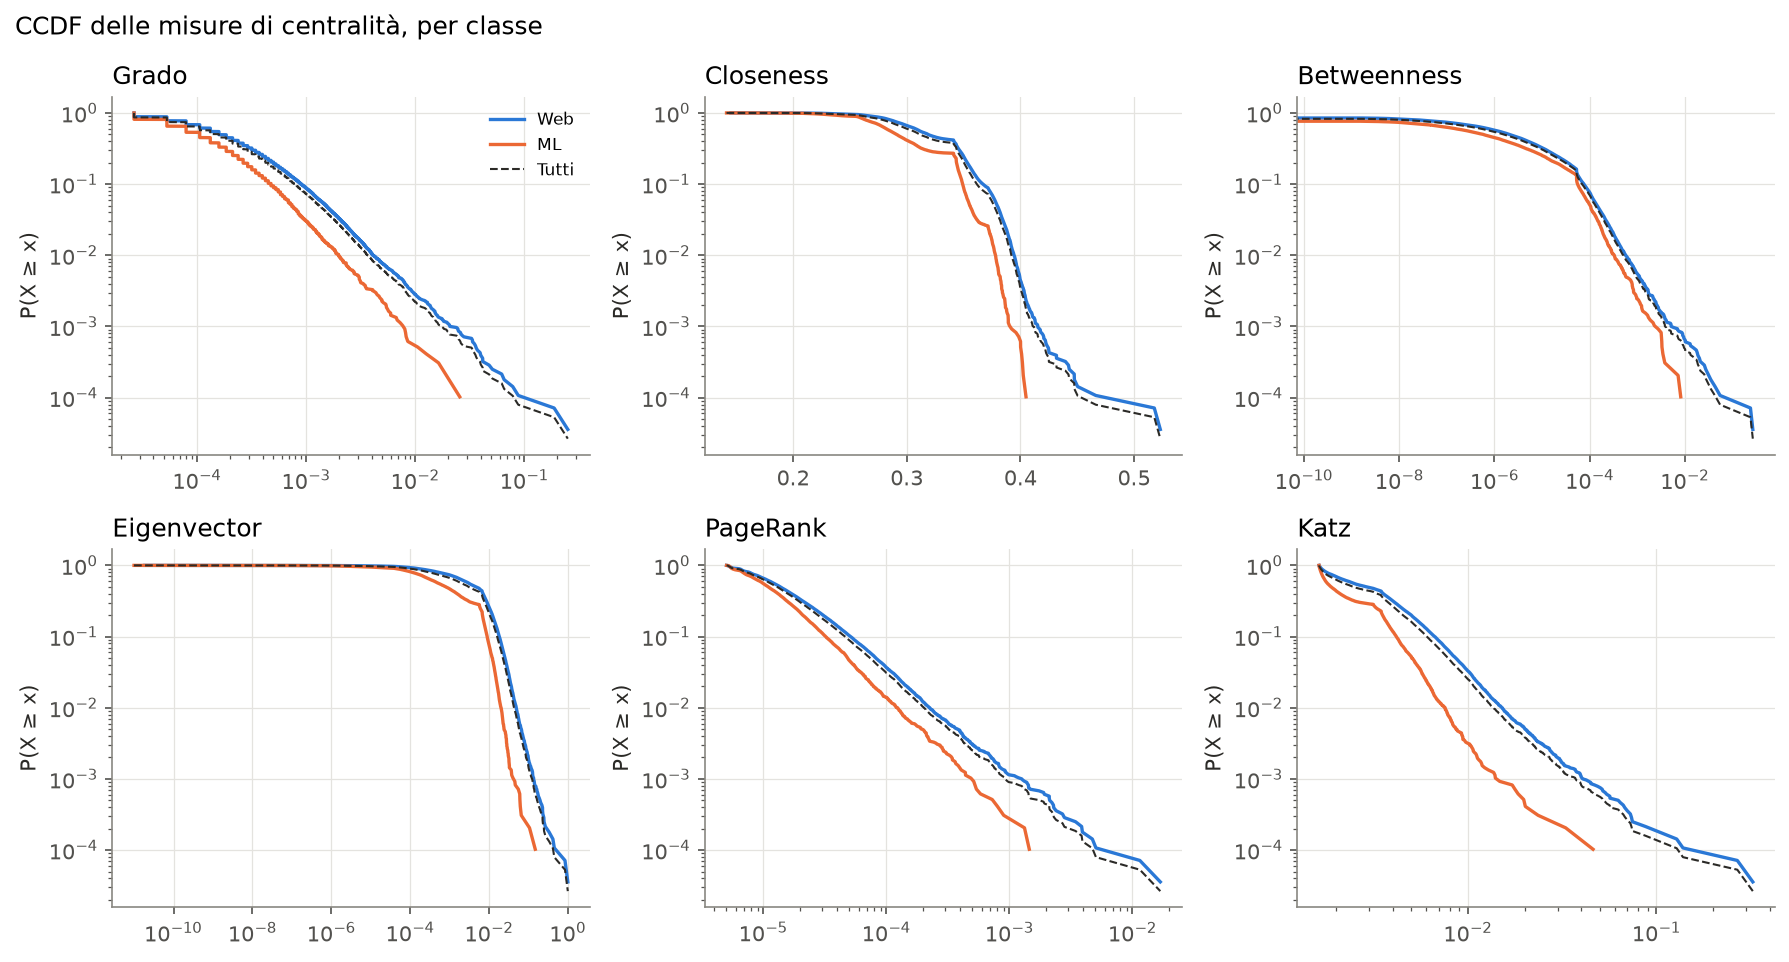
\includegraphics[width=\textwidth]{../2_CENTRALITY_ANALYSIS/figures/01_ccdf_centralita.png}
  \caption{Funzione di distribuzione complementare (CCDF) delle sei misure, per
  l'intera rete e separatamente per sviluppatori web e ML. Scala logaritmica
  (lineare sull'asse delle ascisse per la closeness).}
  \label{fig:ce_ccdf}
\end{figure}

La Figura~\ref{fig:ce_ccdf} e la Tabella~\ref{tab:ce_statistiche} mostrano due
comportamenti molto diversi.
\begin{itemize}
  \item \textbf{Grado, betweenness, PageRank ed eigenvector} hanno distribuzioni a
        coda pesante, quasi rettilinee in scala log-log, ereditate dalla
        distribuzione dei gradi. La betweenness è la più estrema: il nodo più
        centrale ha un valore \num{176000} volte la mediana, il Gini è
        \num{0.93} e il \SI{17}{\percent} dei nodi ha betweenness nulla, cioè non
        si trova su nessun cammino minimo tra altri due nodi (sono soprattutto i
        nodi di grado 1).
  \item \textbf{La closeness} è invece quasi uniforme (Gini \num{0.07}): il
        massimo è appena \num{1.7} volte la mediana. In una rete in cui la distanza
        media è di circa 3,3 passi, anche un nodo periferico raggiunge tutti gli
        altri in pochi passi, e la closeness distingue poco tra i nodi.
\end{itemize}

\subsection{Centralizzazione}
La \textbf{centralizzazione di Freeman} misura quanto l'intera rete è organizzata
attorno a un singolo nodo:
\[
  C_X = \frac{\sum_i \left[C_X(i^*) - C_X(i)\right]}{\max_{G'} \sum_i \left[C_X(i^*) - C_X(i)\right]},
\]
dove $i^*$ è il nodo più centrale e il denominatore è il valore raggiunto dal grafo
a stella con lo stesso numero di nodi, che è il grafo più centralizzato possibile.
Vale quindi 1 per una stella e 0 per un grafo in cui tutti i nodi sono
equivalenti. Si ottiene $C_D=\num{0.25}$ per il grado, $C_B=\num{0.27}$ per la
betweenness e $C_C=\num{0.42}$ per la closeness. Valori di questo ordine sono alti
per una rete di quasi \num{38000} nodi: un solo sviluppatore,
\texttt{dalinhuang99}, è collegato al \SI{25}{\percent} della rete e si trova sul
\SI{27}{\percent} dei cammini minimi.

% ------------------------------------------------------------
\section{I nodi più centrali}
\label{sec:ce_top}

\begin{figure}[H]
  \centering
  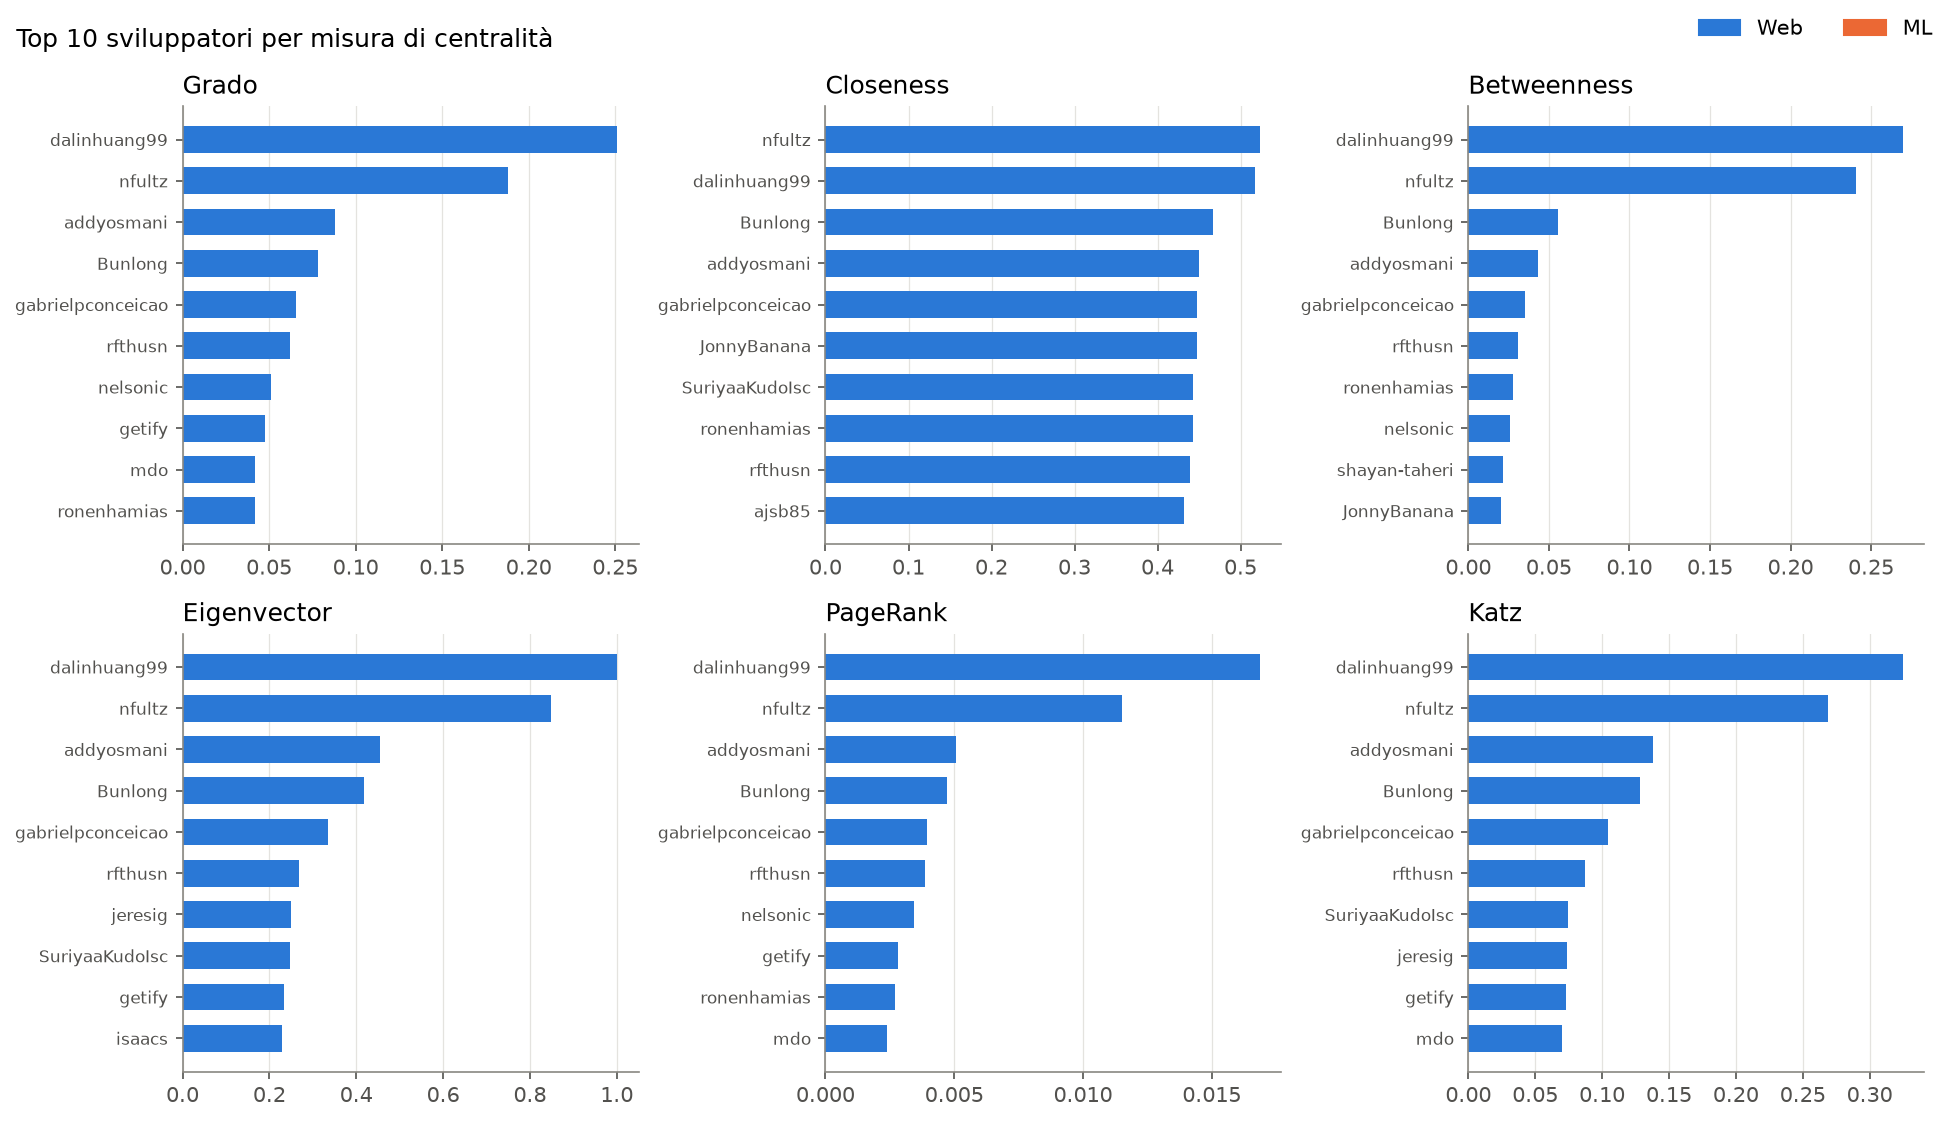
\includegraphics[width=\textwidth]{../2_CENTRALITY_ANALYSIS/figures/02_top10_per_misura.png}
  \caption{I dieci sviluppatori più centrali secondo ciascuna misura. Il colore
  indica la classe; nessuno sviluppatore ML compare in queste classifiche.}
  \label{fig:ce_top10}
\end{figure}

La Figura~\ref{fig:ce_top10} mostra che i vertici delle classifiche sono molto
stabili: \texttt{dalinhuang99} (\num{9458} vicini) e \texttt{nfultz} (\num{7085})
occupano le prime due posizioni per tutte le misure, e i primi sei nodi
(\texttt{dalinhuang99}, \texttt{nfultz}, \texttt{addyosmani}, \texttt{Bunlong},
\texttt{gabrielpconceicao}, \texttt{rfthusn}) sono gli stessi per tutte le misure
tranne la closeness. Si tratta di \emph{hub} con migliaia di contatti, quasi tutti
nodi periferici: il loro coefficiente di clustering è inferiore a \num{0.01}.

Le differenze emergono scendendo nella classifica. Due esempi:
\begin{itemize}
  \item \texttt{nelsonic} è settimo per grado e per PageRank, ma solo 68\textsuperscript{o}
        per closeness: ha molti contatti, ma la sua posizione è più lontana dal
        nucleo della rete, quindi è un hub ``locale'';
  \item \texttt{ajsb85} ha ``solo'' 905 vicini (28\textsuperscript{o} per grado)
        ma è decimo per closeness: pur con meno contatti, si trova in una posizione
        più vicina al nucleo della rete.
\end{itemize}

Nessuno sviluppatore ML compare tra i primi dieci di alcuna misura. Restringendo la
classifica ai soli nodi ML, i più centrali sono \texttt{antirez} (967 vicini,
21\textsuperscript{o} per PageRank nella classifica globale), \texttt{rasbt}
(729 vicini, primo nodo ML per betweenness, 24\textsuperscript{o} globale),
\texttt{bradfitz}, \texttt{amueller} e \texttt{sebastianruder}.

% ------------------------------------------------------------
\section{Confronto tra le misure}
\label{sec:ce_correlazioni}

Per confrontare le misure si usano due strumenti complementari:
\begin{itemize}
  \item la \textbf{correlazione di Spearman}, calcolata sui ranghi di tutti i nodi,
        che misura l'accordo sull'intera classifica;
  \item l'\textbf{indice di Jaccard} tra gli insiemi dei 100 nodi più centrali,
        $J(A,B)=|A\cap B|/|A\cup B|$, che misura l'accordo sul vertice della
        classifica, cioè sui nodi che di solito interessano.
\end{itemize}

\begin{figure}[H]
  \centering
  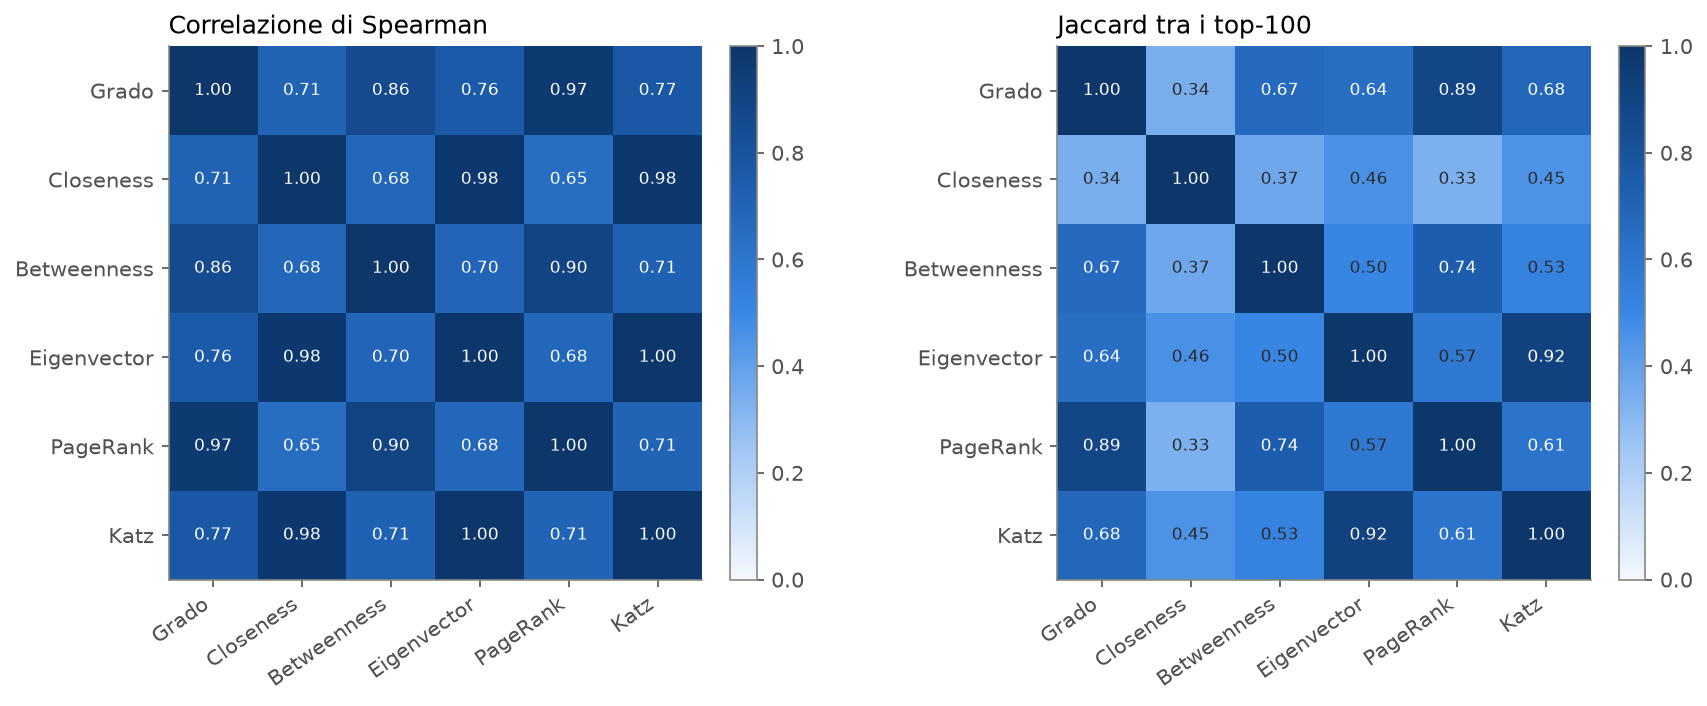
\includegraphics[width=\textwidth]{../2_CENTRALITY_ANALYSIS/figures/03_correlazioni_overlap.png}
  \caption{A sinistra, correlazione di Spearman tra le misure; a destra, indice di
  Jaccard tra i 100 nodi più centrali per ciascuna misura.}
  \label{fig:ce_correlazioni}
\end{figure}

\begin{figure}[H]
  \centering
  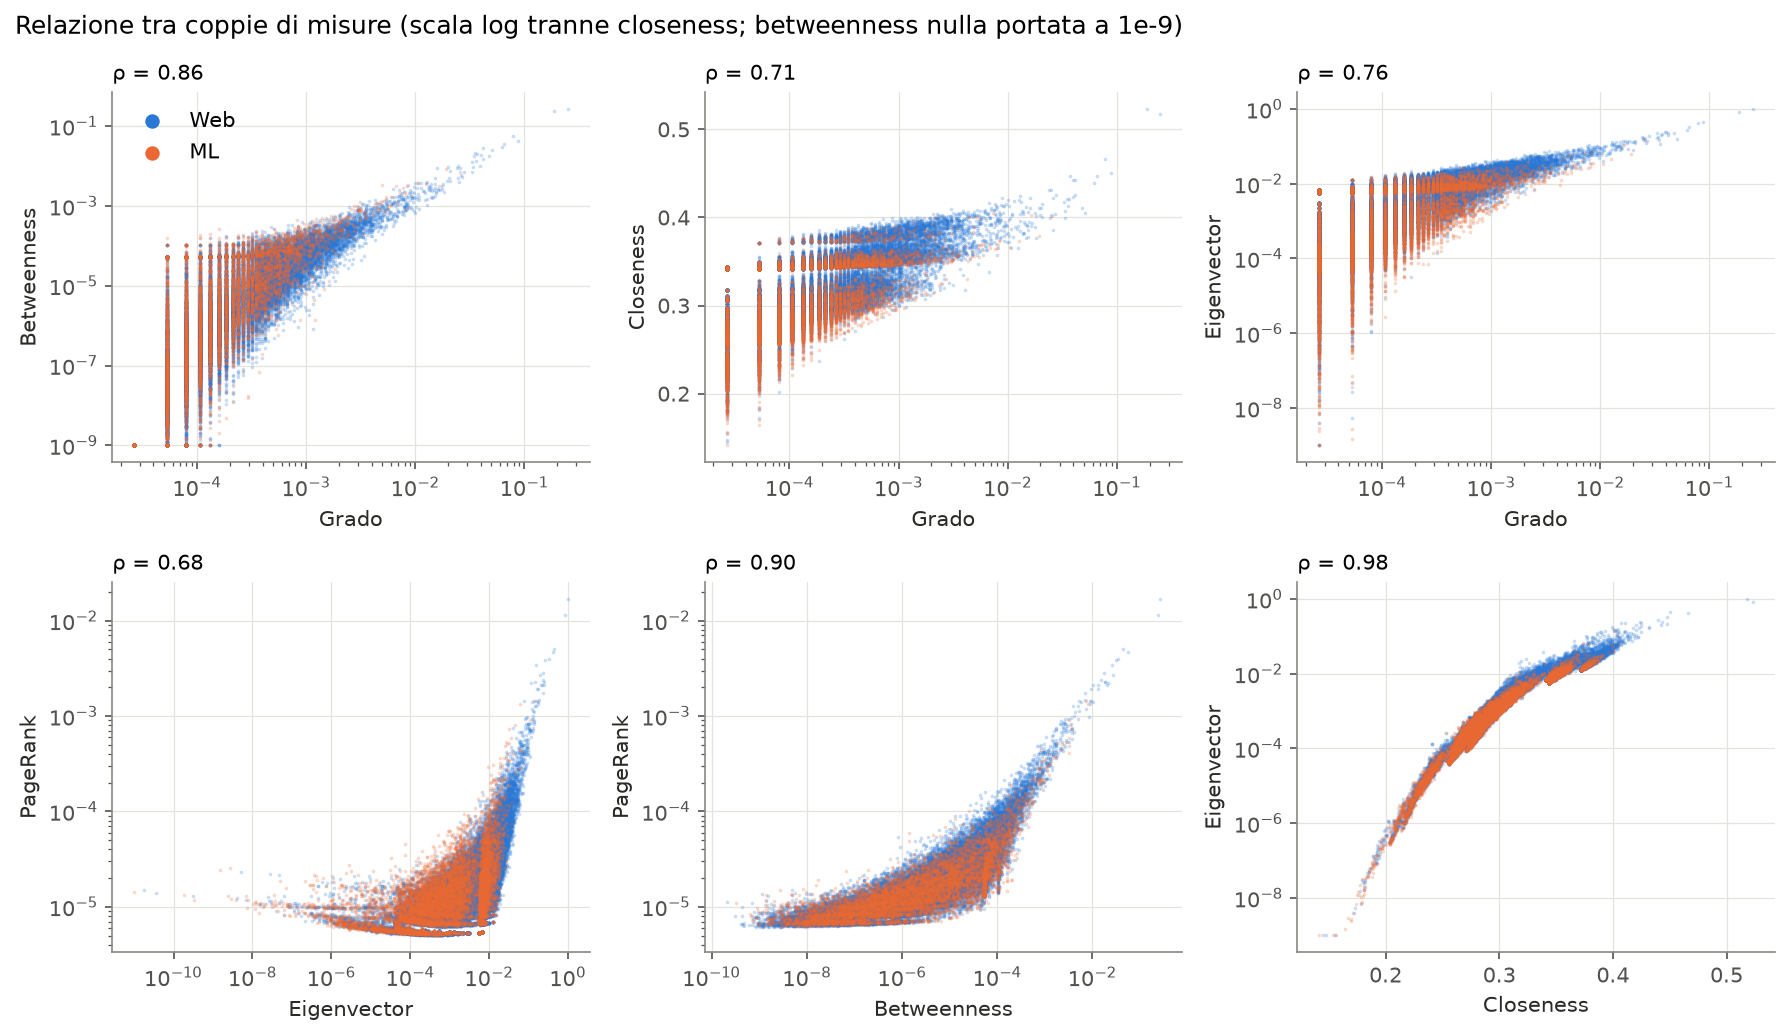
\includegraphics[width=\textwidth]{../2_CENTRALITY_ANALYSIS/figures/04_scatter_coppie.png}
  \caption{Relazione tra coppie di misure; ogni punto è uno sviluppatore. $\rho$ è
  la correlazione di Spearman.}
  \label{fig:ce_scatter}
\end{figure}

Le Figure~\ref{fig:ce_correlazioni} e~\ref{fig:ce_scatter} mostrano che le misure
formano due gruppi.
\begin{itemize}
  \item \textbf{Grado, PageRank e betweenness}: Spearman tra \num{0.86} e
        \num{0.97}. PageRank su un grafo non orientato è quasi proporzionale al
        grado, a meno del termine di teletrasporto ($\rho=\num{0.97}$, Jaccard
        \num{0.89}). Anche la betweenness segue da vicino il grado: un nodo con
        molti vicini a basso grado è necessariamente sui cammini minimi tra di essi.
  \item \textbf{Closeness, eigenvector e Katz}: Spearman tra \num{0.98} e
        \num{0.999}. Eigenvector e Katz sono quasi identiche ($\rho=\num{0.999}$),
        perché con $\alpha$ relativamente vicino a $1/\lambda_{\max}$ la centralità di Katz tende
        all'autovettore dominante. Queste misure premiano la vicinanza al nucleo
        della rete più che il numero di contatti.
\end{itemize}
Tra i due gruppi la correlazione scende a circa \num{0.65}--\num{0.77}, e la
sovrapposizione minima tra i top-100 si ha tra closeness e PageRank (Jaccard
\num{0.33}). Il grafico grado--betweenness della Figura~\ref{fig:ce_scatter} mostra
inoltre che, a parità di grado, la betweenness varia di diversi ordini di grandezza:
è il segnale della presenza di nodi \emph{ponte}.

\subsection{Nodi ponte}
Un nodo con betweenness alta rispetto al proprio grado collega zone della rete che
altrimenti sarebbero lontane. Tra i primi 1000 nodi per betweenness, si sono
cercati quelli che guadagnano più posizioni rispetto alla classifica per grado. Il
caso più estremo è \texttt{artificialsoph}: ha solo 6 vicini (posizione
\num{17063} per grado) ma è 821\textsuperscript{o} per betweenness. Ha
clustering nullo, cioè nessuno dei suoi vicini è collegato agli altri, e
\SI{83}{\percent} dei suoi vicini sono sviluppatori ML: è un punto di accesso
dell'area ML al resto della rete. Gli altri nodi ponte hanno caratteristiche
simili: grado tra 13 e 28, clustering basso e vicini di entrambe le classi.

% ------------------------------------------------------------
\section{Centralità e classe}
\label{sec:ce_classe}

Il dataset classifica ogni sviluppatore come web (\SI{74.2}{\percent}) o machine
learning (\SI{25.8}{\percent}). Per verificare se le due classi occupano posizioni
diverse nella rete, per ciascuna misura si è applicato il \textbf{test di
Mann--Whitney U}, che non richiede ipotesi sulla forma delle distribuzioni. Oltre
al p-value si riporta la statistica normalizzata
$U/(n_{\text{web}}\,n_{\text{ML}})$, che stima la probabilità che uno sviluppatore
web scelto a caso sia più centrale di uno ML scelto a caso: 0,5 indica nessuna
differenza (Tabella~\ref{tab:ce_classe}).

\begin{table}[H]
  \centering
  \caption{Centralità per classe. Il rapporto è calcolato tra le mediane.}
  \label{tab:ce_classe}
  \small
  \begin{tabular}{@{}lrrrrr@{}}
    \toprule
    \textbf{Misura} & \textbf{Med.\ web} & \textbf{Med.\ ML} & \textbf{Rapporto} & \textbf{P(web $>$ ML)} & \textbf{ML top-100} \\
    \midrule
    Grado       & \num{1.59e-4} & \num{1.06e-4} & \num{1.50} & \num{0.61} & \SI{5}{\percent} \\
    Closeness   & \num{0.319}   & \num{0.291}   & \num{1.10} & \num{0.66} & \SI{2}{\percent} \\
    Betweenness & \num{2.04e-6} & \num{5.72e-7} & \num{3.56} & \num{0.57} & \SI{13}{\percent} \\
    Eigenvector & \num{4.63e-3} & \num{8.03e-4} & \num{5.77} & \num{0.68} & \SI{2}{\percent} \\
    PageRank    & \num{1.38e-5} & \num{1.10e-5} & \num{1.25} & \num{0.58} & \SI{10}{\percent} \\
    Katz        & \num{2.90e-3} & \num{1.88e-3} & \num{1.54} & \num{0.67} & \SI{3}{\percent} \\
    \bottomrule
  \end{tabular}
\end{table}

\begin{figure}[H]
  \centering
  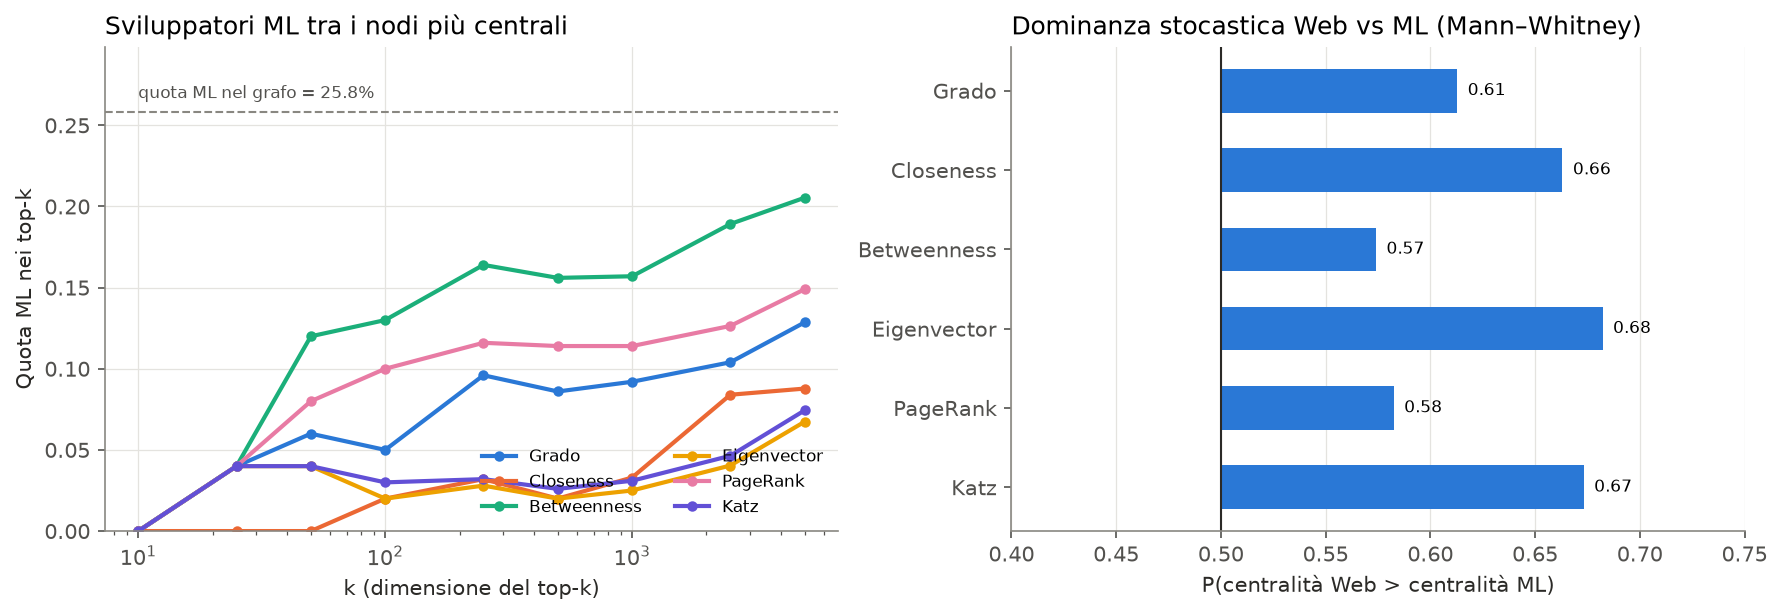
\includegraphics[width=\textwidth]{../2_CENTRALITY_ANALYSIS/figures/05_centralita_per_classe.png}
  \caption{A sinistra, quota di sviluppatori ML tra i $k$ nodi più centrali al
  variare di $k$ (la linea tratteggiata è la quota nell'intera rete); a destra,
  probabilità che un nodo web sia più centrale di un nodo ML.}
  \label{fig:ce_classe}
\end{figure}

Per tutte le misure gli sviluppatori web sono significativamente più centrali (i
p-value sono tutti inferiori a $10^{-100}$). L'effetto però non è uniforme
(Figura~\ref{fig:ce_classe}).
\begin{itemize}
  \item È massimo per \textbf{eigenvector, Katz e closeness} (probabilità
        \num{0.67}--\num{0.68}): le misure che premiano la vicinanza al nucleo
        della rete penalizzano gli sviluppatori ML, che formano un'area propria e
        periferica. Tra i primi 100 nodi per eigenvector gli sviluppatori ML sono
        solo il \SI{2}{\percent}, contro il \SI{25.8}{\percent} della rete.
  \item È minimo per \textbf{betweenness e PageRank} (\num{0.57}--\num{0.58}). In
        particolare la betweenness è la misura in cui gli sviluppatori ML sono più
        rappresentati al vertice (\SI{13}{\percent} dei top-100,
        \SI{20.5}{\percent} dei top-\num{5000}): i pochi nodi ML ben collegati
        fanno da ponte tra l'area ML e il resto della rete, e attirano quindi
        molti cammini minimi.
\end{itemize}

% ------------------------------------------------------------
\section{Robustezza della rete}
\label{sec:ce_robustezza}

Un modo per verificare se le misure individuano davvero i nodi importanti è
osservare cosa succede alla rete quando questi vengono rimossi. Per ciascuna misura
si sono rimossi i nodi più centrali, dallo \SI{0.25}{\percent} al
\SI{5}{\percent} del totale, misurando la dimensione della componente connessa
più grande e il numero di componenti. L'ordine di rimozione è calcolato una sola
volta sulla rete intatta. Come riferimento si è usata la rimozione di nodi scelti a
caso.

\begin{figure}[H]
  \centering
  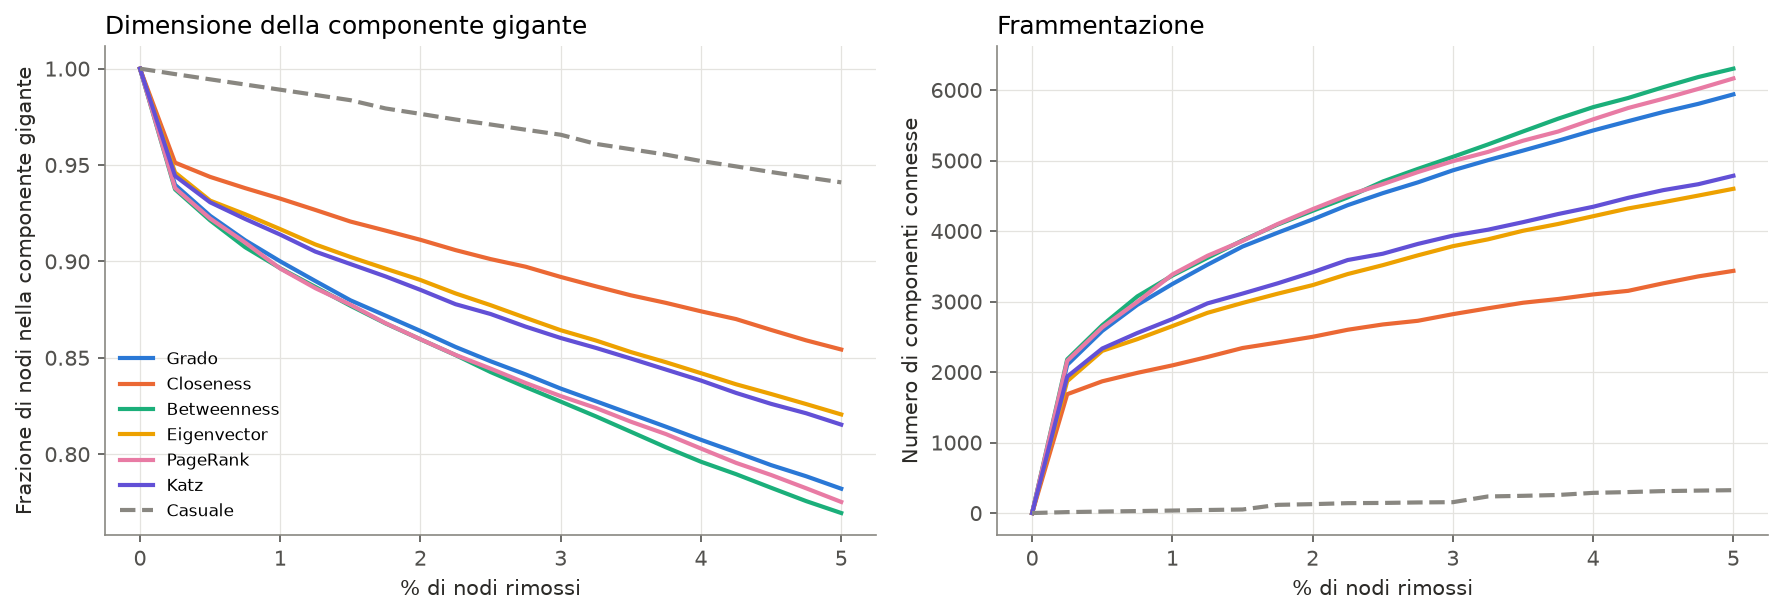
\includegraphics[width=\textwidth]{../2_CENTRALITY_ANALYSIS/figures/06_robustezza_rimozione.png}
  \caption{Effetto della rimozione dei nodi più centrali, confrontata con la
  rimozione casuale. A sinistra, frazione dei nodi (sul totale iniziale) che resta
  nella componente gigante; a destra, numero di componenti connesse.}
  \label{fig:ce_robustezza}
\end{figure}

La Figura~\ref{fig:ce_robustezza} mostra il comportamento tipico delle reti con
distribuzione dei gradi a coda pesante: \textbf{robuste ai guasti casuali, fragili
agli attacchi mirati}.
\begin{itemize}
  \item Rimuovendo il \SI{5}{\percent} dei nodi a caso, la componente gigante
        contiene ancora il \SI{94.1}{\percent} dei nodi: si perdono quasi
        soltanto i nodi rimossi.
  \item Rimuovendo lo stesso numero di nodi in ordine di betweenness, la
        componente gigante scende al \SI{77.0}{\percent} e la rete si frammenta in
        oltre \num{6000} componenti. Già la rimozione dello \SI{0.25}{\percent}
        dei nodi (94 sviluppatori) stacca dalla rete circa \num{2000} componenti,
        formate in gran parte dai nodi che erano collegati solo agli hub rimossi.
  \item Le misure più efficaci sono betweenness, PageRank e grado; la closeness è
        la meno efficace (\SI{85.4}{\percent} dopo il \SI{5}{\percent} di
        rimozioni), perché premia i nodi vicini al nucleo, non quelli da cui
        dipende la periferia.
\end{itemize}

% ------------------------------------------------------------
\section{Visualizzazione dei nodi più centrali}
\label{sec:ce_visualizzazione}

\begin{figure}[H]
  \centering
  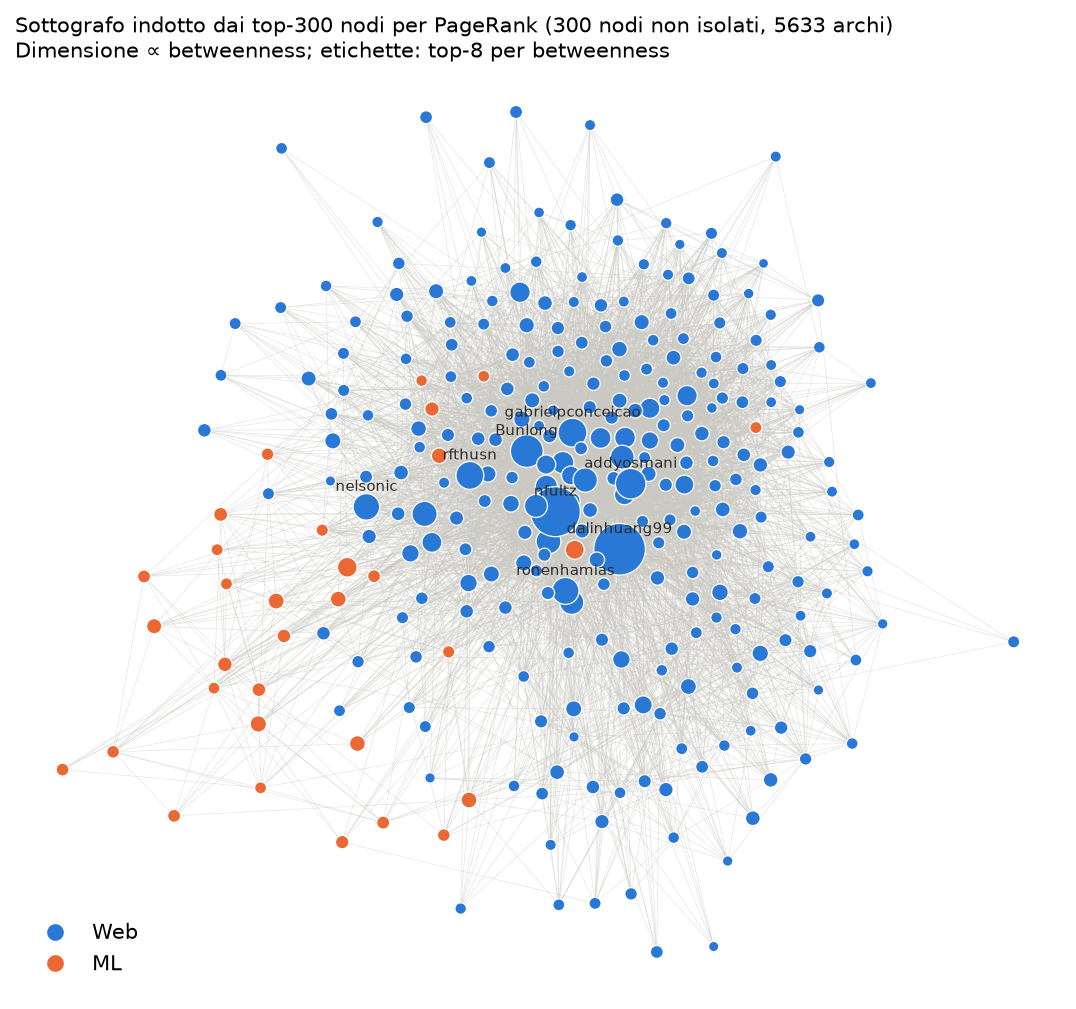
\includegraphics[width=0.85\textwidth]{../2_CENTRALITY_ANALYSIS/figures/07_sottografo_top_pagerank.png}
  \caption{Sottografo indotto dai 300 nodi con PageRank più alto, disposto con
  l'algoritmo di Fruchterman--Reingold. La dimensione dei nodi è proporzionale
  alla betweenness, il colore indica la classe.}
  \label{fig:ce_sottografo}
\end{figure}

La Figura~\ref{fig:ce_sottografo} mostra le relazioni tra i 300 nodi con PageRank
più alto. I nodi sono tutti collegati tra loro (nessuno è isolato nel sottografo) e
formano un nucleo denso di sviluppatori web, con i grandi hub al centro. I pochi
sviluppatori ML presenti si raggruppano invece in un settore separato, ai margini
del nucleo: anche al vertice della rete le due classi restano in gran parte
distinte, come si vedrà con l'analisi delle community
(Capitolo~\ref{cap:strutture}).

% ------------------------------------------------------------
\section{Conclusioni}
\label{sec:ce_conclusioni}

\begin{itemize}
  \item La centralità è \textbf{fortemente concentrata}: pochi hub, in particolare
        \texttt{dalinhuang99} e \texttt{nfultz}, occupano i primi posti di tutte le
        classifiche e si trovano, rispettivamente, sul \SI{27}{\percent} e sul
        \SI{24}{\percent} dei cammini minimi della rete.
  \item Le misure sono molto correlate nel complesso, ma si dividono in due gruppi:
        grado, PageRank e betweenness misurano il \emph{numero} di contatti;
        closeness, eigenvector e Katz la \emph{posizione} rispetto al nucleo della
        rete. La scelta della misura cambia soprattutto la parte alta della
        classifica.
  \item Gli \textbf{sviluppatori ML sono sistematicamente meno centrali} degli
        sviluppatori web, soprattutto secondo le misure spettrali. Fa eccezione la
        betweenness, che premia i nodi ML che fanno da ponte verso il resto della
        rete.
  \item La rete è \textbf{robusta ai guasti casuali ma fragile agli attacchi
        mirati}: dopo la rimozione del \SI{5}{\percent} dei nodi più centrali la
        componente gigante contiene circa il \SI{77}{\percent} dei nodi, contro
        il \SI{94}{\percent} dopo una rimozione casuale.
\end{itemize}

% ==================== CAPITOLO 4 - VISUALIZZAZIONE E ANALISI DELLE STRUTTURE ====================
\chapter{Visualizzazione e analisi delle strutture}
\label{cap:strutture}

% ------------------------------------------------------------
\section{Introduzione}
\label{sec:st_intro}

Il capitolo precedente ha studiato l'importanza dei singoli nodi. Questo capitolo
studia invece l'\textbf{organizzazione complessiva} della rete, a diverse scale:
\begin{itemize}
  \item i punti critici per la connettività (Sezione~\ref{sec:st_connettivita});
  \item la struttura a strati nucleo--periferia, tramite la decomposizione
        $k$-core (Sezione~\ref{sec:st_kcore});
  \item i gruppi completamente connessi, cioè le clique (Sezione~\ref{sec:st_clique});
  \item le proprietà \emph{small-world}, confrontando la rete con grafi casuali
        (Sezione~\ref{sec:st_smallworld});
  \item la tendenza degli hub a collegarsi tra loro, cioè il fenomeno del
        \emph{rich-club} (Sezione~\ref{sec:st_richclub});
  \item la suddivisione in community (Sezione~\ref{sec:st_community});
  \item la visualizzazione dell'intera rete (Sezione~\ref{sec:st_visualizzazione}).
\end{itemize}
In ogni sezione si verifica anche il rapporto tra la struttura trovata e la classe
degli sviluppatori (web o ML).

\subsection{Librerie utilizzate}
{\sloppy Il codice è contenuto nello script \texttt{structure\_analysis.py}
(cartella \texttt{3\_STRUCTURE\_ANALYSIS/codice}), che utilizza le seguenti
librerie:\par}
\begin{itemize}
  \item \textbf{python-igraph}: rappresentazione del grafo, $k$-core, clique,
        generazione dei grafi casuali, algoritmi di community detection e layout;
  \item \textbf{leidenalg}: algoritmo di Leiden;
  \item \textbf{SciPy}, \textbf{pandas} e \textbf{NumPy}: statistiche e gestione
        dei risultati;
  \item \textbf{Matplotlib}: realizzazione dei grafici.
\end{itemize}
Le partizioni in community e il layout della rete completa vengono salvati nella
cartella \texttt{cache}. Le tabelle complete sono raccolte nel file
\texttt{structure\_results.md}.

% ------------------------------------------------------------
\section{Connettività e punti critici}
\label{sec:st_connettivita}

La rete è formata da un'unica componente connessa. La connessione però è fragile in
molti punti:
\begin{itemize}
  \item un \textbf{punto di articolazione} è un nodo la cui rimozione disconnette
        il grafo: ce ne sono \num{3188}, l'\SI{8.5}{\percent} dei nodi;
  \item un \textbf{bridge} è un arco la cui rimozione disconnette il grafo: ce ne
        sono \num{5241}.
\end{itemize}
Quasi tutti i bridge (\num{5045} su \num{5241}) collegano un nodo di grado 1 al
resto della rete. La rete ha quindi una struttura a due livelli: un
\textbf{nucleo biconnesso}, in cui ogni nodo resta raggiungibile anche dopo la
rimozione di un qualsiasi altro nodo, che contiene \num{32416} nodi
(\SI{86}{\percent}), e una periferia di nodi ``appesi'' al nucleo. La seconda
componente biconnessa più grande ha appena 4 nodi.

I punti di articolazione più importanti sono i grandi hub del
Capitolo~\ref{cap:centralita}. Rimuovendo \texttt{dalinhuang99} la rete si spezza in
369 componenti e si staccano 379 nodi, collegati alla rete solo attraverso di lui;
rimuovendo \texttt{nfultz} se ne staccano 123.

% ------------------------------------------------------------
\section{Decomposizione $k$-core}
\label{sec:st_kcore}

Il \textbf{$k$-core} di un grafo è il sottografo massimale in cui ogni nodo ha
almeno $k$ vicini all'interno del sottografo stesso. Si ottiene eliminando
ripetutamente i nodi di grado inferiore a $k$. La \textbf{coreness} di un nodo è il
massimo $k$ per cui il nodo appartiene al $k$-core, e l'insieme dei nodi con
coreness esattamente $k$ forma la $k$-\emph{shell}. A differenza del grado, la
coreness misura se un nodo è inserito in una zona densa della rete: un hub collegato
solo a nodi periferici ha grado alto ma coreness bassa.

\begin{figure}[H]
  \centering
  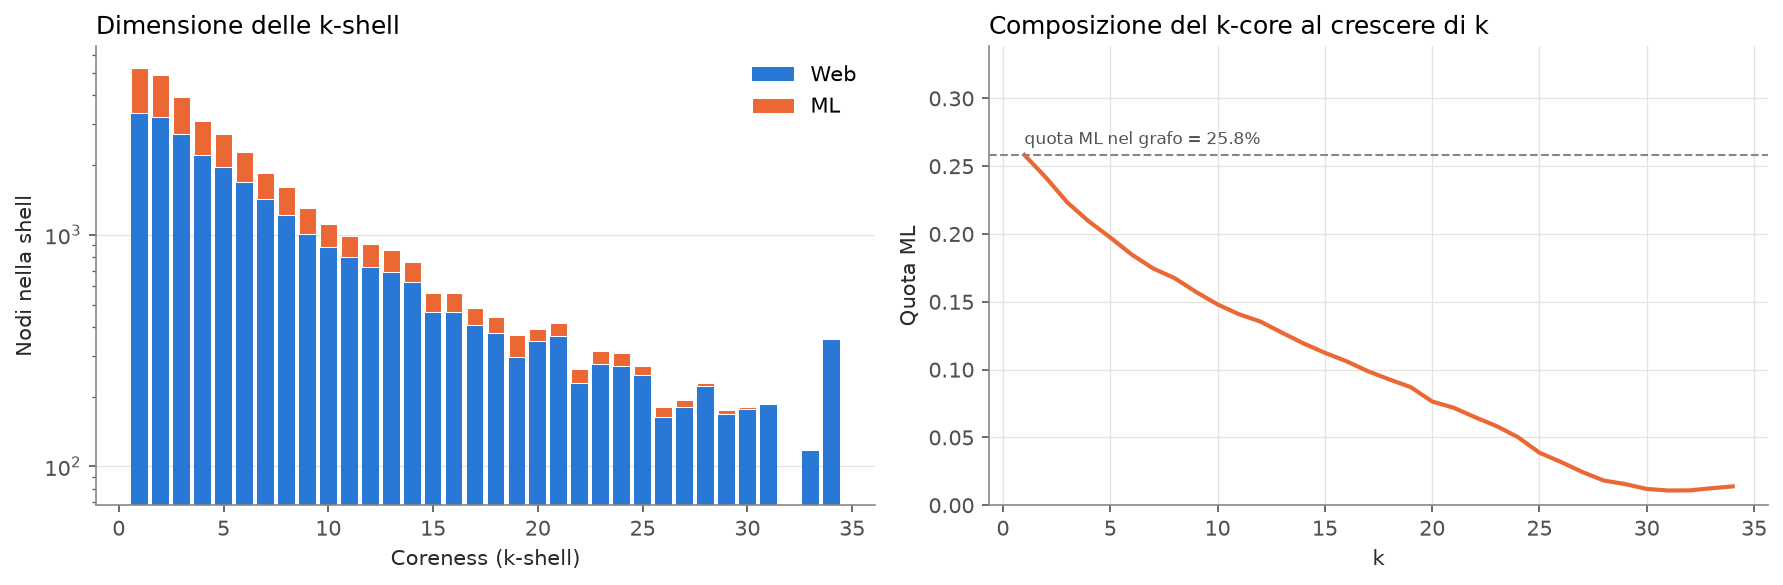
\includegraphics[width=\textwidth]{../3_STRUCTURE_ANALYSIS/figures/01_kcore.png}
  \caption{A sinistra, numero di nodi in ciascuna $k$-shell, suddivisi per classe
  (scala logaritmica); a destra, quota di sviluppatori ML nel $k$-core al
  crescere di $k$.}
  \label{fig:st_kcore}
\end{figure}

\begin{table}[H]
  \centering
  \caption{Dimensione e composizione del $k$-core.}
  \label{tab:st_kcore}
  \small
  \begin{tabular}{@{}rrrr@{}}
    \toprule
    $k$ & \textbf{Nodi nel $k$-core} & \textbf{Quota della rete} & \textbf{Quota ML} \\
    \midrule
    1  & \num{37700} & \SI{100}{\percent}  & \SI{25.8}{\percent} \\
    2  & \num{32464} & \SI{86.1}{\percent} & \SI{24.2}{\percent} \\
    5  & \num{20491} & \SI{54.4}{\percent} & \SI{19.8}{\percent} \\
    10 & \num{10710} & \SI{28.4}{\percent} & \SI{14.8}{\percent} \\
    20 & \num{3661}  & \SI{9.7}{\percent}  & \SI{7.6}{\percent} \\
    30 & \num{915}   & \SI{2.4}{\percent}  & \SI{1.2}{\percent} \\
    34 & \num{360}   & \SI{1.0}{\percent}  & \SI{1.4}{\percent} \\
    \bottomrule
  \end{tabular}
\end{table}

La coreness massima è $k_{\max}=34$. Il 34-core, il nucleo più interno della rete,
contiene 360 nodi e \num{10488} archi, con densità \num{0.16}: circa 400 volte
quella dell'intera rete. La Figura~\ref{fig:st_kcore} mostra che la dimensione delle
shell decresce regolarmente con $k$, ma l'ultima shell è più popolata delle
precedenti: il nucleo è un gruppo compatto, distinto dalla periferia.

La composizione per classe è il risultato più netto
(Tabella~\ref{tab:st_kcore}). La quota di sviluppatori ML diminuisce in modo
praticamente monotono con $k$: dal \SI{25.8}{\percent} dell'intera rete all'\SI{1.4}{\percent}
del nucleo. La coreness mediana è 6 per gli sviluppatori web e 4 per quelli ML. Il
nucleo della rete è quindi formato quasi esclusivamente da sviluppatori web,
coerentemente con le misure di centralità spettrali del
Capitolo~\ref{cap:centralita}.

% ------------------------------------------------------------
\section{Clique}
\label{sec:st_clique}

Una \textbf{clique} è un insieme di nodi tutti collegati tra loro; è
\textbf{massimale} se non può essere estesa aggiungendo un altro nodo. Trovare
tutte le clique massimali è un problema NP-difficile nel caso generale, ma su una
rete sparsa come questa l'algoritmo di igraph impiega circa 1,5 secondi.

\begin{figure}[H]
  \centering
  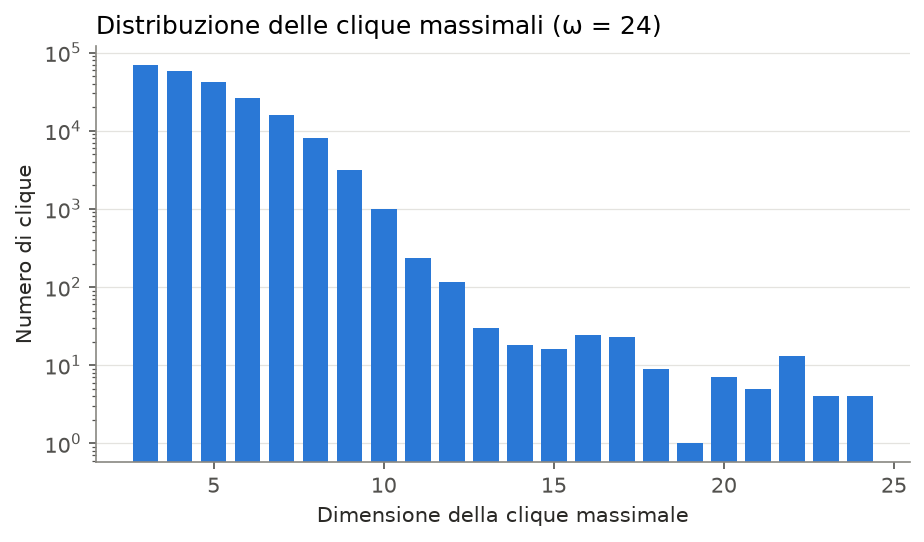
\includegraphics[width=0.75\textwidth]{../3_STRUCTURE_ANALYSIS/figures/02_clique.png}
  \caption{Distribuzione della dimensione delle clique massimali (scala
  logaritmica).}
  \label{fig:st_clique}
\end{figure}

La rete contiene \num{223672} clique massimali con almeno 3 nodi
(Figura~\ref{fig:st_clique}). La clique più grande ha $\omega(G)=24$ nodi; le
quattro clique di dimensione massima coinvolgono in tutto 26 nodi e ne condividono
22, quindi sono varianti dello stesso gruppo di sviluppatori, quasi tutti web
(\SI{3.8}{\percent} ML).

\begin{table}[H]
  \centering
  \caption{Composizione per classe delle clique massimali.}
  \label{tab:st_clique}
  \small
  \begin{tabular}{@{}lrrrr@{}}
    \toprule
    \textbf{Dimensione} & \textbf{Clique} & \textbf{Solo web} & \textbf{Solo ML} & \textbf{Miste} \\
    \midrule
    $\geq 3$  & \num{223672} & \SI{82.2}{\percent} & \SI{1.3}{\percent}  & \SI{16.4}{\percent} \\
    $\geq 5$  & \num{96944}  & \SI{87.9}{\percent} & \SI{0.1}{\percent}  & \SI{12.0}{\percent} \\
    $\geq 10$ & \num{1496}   & \SI{65.7}{\percent} & \SI{0}{\percent}    & \SI{34.3}{\percent} \\
    $\geq 15$ & \num{106}    & \SI{39.6}{\percent} & \SI{0}{\percent}    & \SI{60.4}{\percent} \\
    \bottomrule
  \end{tabular}
\end{table}

La Tabella~\ref{tab:st_clique} mostra che le clique composte da soli sviluppatori
ML sono rare e piccole: nessuna clique con almeno 10 nodi è interamente ML. Le
clique grandi sono invece sempre più spesso miste: gli sviluppatori ML partecipano
ai gruppi densi soprattutto insieme a sviluppatori web.

% ------------------------------------------------------------
\section{Small-world e confronto con modelli nulli}
\label{sec:st_smallworld}

Una rete è detta \textbf{small-world} se ha distanze medie brevi, come un grafo
casuale, ma un clustering molto più alto. Per verificarlo, la rete è stata
confrontata con due \textbf{modelli nulli}, cioè grafi casuali che conservano solo
alcune proprietà della rete reale:
\begin{itemize}
  \item il grafo di \textbf{Erdős--Rényi} $G(n,m)$, con lo stesso numero di nodi e
        di archi, archi scelti in modo uniforme;
  \item il \textbf{configuration model}, con la stessa sequenza dei gradi della rete
        reale, generato con l'algoritmo di Viger--Latapy (grafo semplice e
        connesso).
\end{itemize}
Il secondo modello permette di capire quali proprietà della rete reale siano una
semplice conseguenza della distribuzione dei gradi e quali no. Per ciascun modello
sono state generate 5 repliche. La distanza media è stimata con visite in ampiezza da
300 nodi sorgente, gli stessi per tutti i grafi.

\begin{table}[H]
  \centering
  \caption{Rete reale e modelli nulli (medie su 5 repliche).}
  \label{tab:st_smallworld}
  \small
  \begin{tabular}{@{}lrrrr@{}}
    \toprule
    \textbf{Grafo} & \textbf{Transitività} & \textbf{Clustering medio} & \textbf{Distanza media} & \textbf{Assortatività} \\
    \midrule
    GitHub (reale)      & \num{0.0124}  & \num{0.1675}  & \num{3.27} & \num{-0.075} \\
    Erdős--Rényi        & \num{0.0004}  & \num{0.0004}  & \num{4.14} & \num{0.001} \\
    Configuration model & \num{0.0123}  & \num{0.0923}  & \num{3.14} & \num{-0.071} \\
    \bottomrule
  \end{tabular}
\end{table}

\begin{figure}[H]
  \centering
  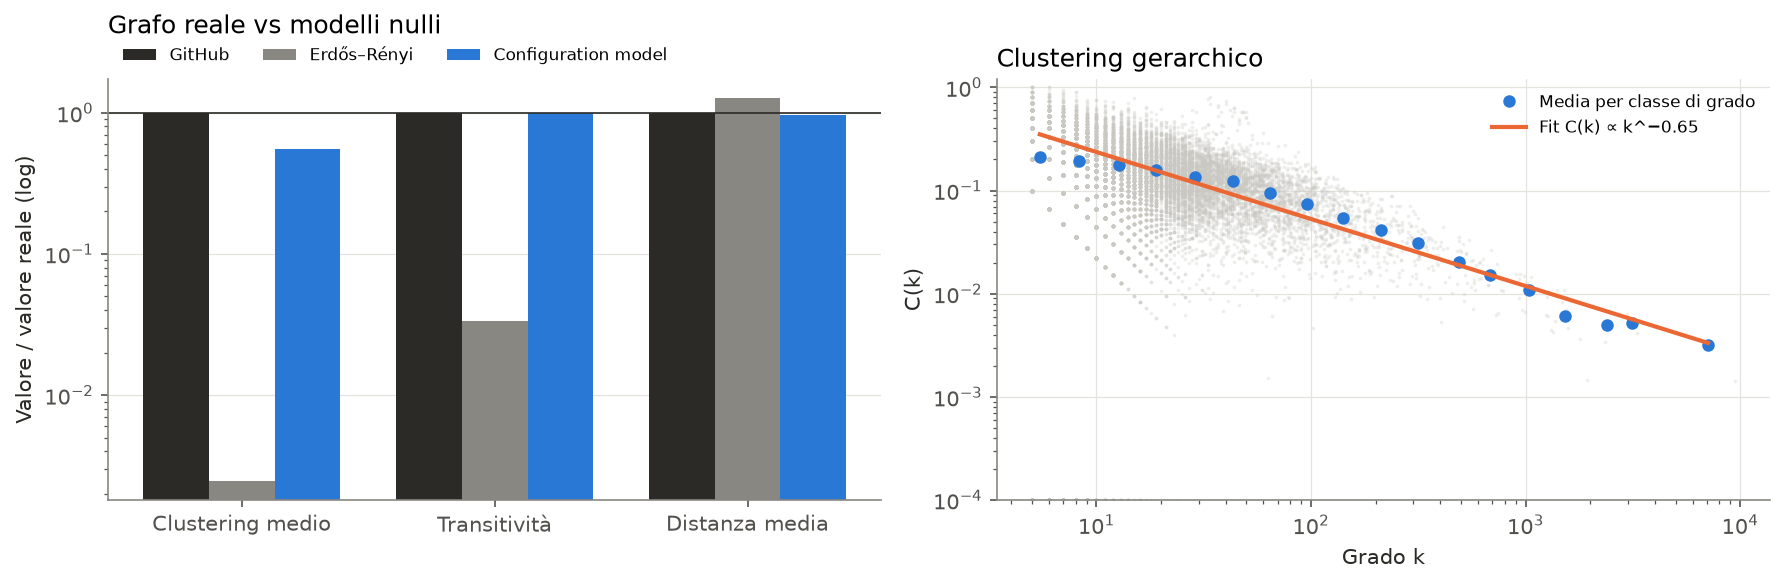
\includegraphics[width=\textwidth]{../3_STRUCTURE_ANALYSIS/figures/03_small_world.png}
  \caption{A sinistra, rapporto tra le proprietà dei modelli nulli e quelle della
  rete reale (scala logaritmica); a destra, clustering locale medio in funzione del
  grado, con retta di regressione in scala log-log.}
  \label{fig:st_smallworld}
\end{figure}

Dalla Tabella~\ref{tab:st_smallworld} e dalla Figura~\ref{fig:st_smallworld}
emergono tre risultati.
\begin{enumerate}
  \item \textbf{La rete è small-world.} La distanza media (\num{3.27}) è persino
        inferiore a quella del grafo di Erdős--Rényi (\num{4.14}), grazie agli hub,
        mentre il clustering medio è circa 400 volte più alto. Il coefficiente
        \[
          \sigma = \frac{C/C_{\text{rand}}}{L/L_{\text{rand}}},
        \]
        dove $C$ è il clustering medio e $L$ la distanza media, vale circa 513
        rispetto a Erdős--Rényi (una rete è small-world se $\sigma>1$).
  \item \textbf{Il configuration model spiega molte proprietà della rete}: la
        transitività, la distanza media e anche la disassortatività di grado sono
        quasi identiche a quelle reali. Sono quindi conseguenze della distribuzione
        dei gradi: gli hub, collegandosi necessariamente a molti nodi di grado
        basso, rendono la rete disassortativa e accorciano le distanze.
  \item \textbf{Il clustering medio no}: quello reale è \num{1.8} volte quello del
        configuration model ($\sigma=\num{1.74}$ rispetto a questo modello). Tra
        gli sviluppatori di grado basso e medio c'è quindi una tendenza a formare
        triangoli (``gli amici dei miei amici sono miei amici'') che la sola
        distribuzione dei gradi non spiega.
\end{enumerate}

Il grafico a destra della Figura~\ref{fig:st_smallworld} mostra infine che il
clustering locale decresce con il grado secondo una legge di potenza
$C(k)\propto k^{-\beta}$ con $\beta=\num{0.65}$ ($R^2=\num{0.97}$). Nei modelli
gerarchici di Ravasz e Barabási si ha $\beta=1$: i nodi di grado basso appartengono
a piccoli gruppi densi, mentre gli hub collegano gruppi diversi e hanno quindi
clustering basso. Il valore osservato indica una struttura gerarchica, anche se meno
marcata di quella del modello teorico.

% ------------------------------------------------------------
\section{Rich-club}
\label{sec:st_richclub}

Il \textbf{coefficiente rich-club} misura se i nodi di grado alto tendono a
collegarsi tra loro:
\[
  \phi(k) = \frac{2E_{>k}}{N_{>k}(N_{>k}-1)},
\]
dove $N_{>k}$ è il numero di nodi con grado maggiore di $k$ ed $E_{>k}$ il numero di
archi tra di essi; $\phi(k)$ è quindi la densità del sottografo dei nodi ``ricchi''.
Poiché $\phi(k)$ cresce con $k$ anche in un grafo casuale, lo si confronta con il
valore medio $\phi_{\text{rand}}(k)$ ottenuto su 5 grafi ricablati che conservano i
gradi. Il coefficiente normalizzato $\rho(k)=\phi(k)/\phi_{\text{rand}}(k)$ è
maggiore di 1 se gli hub si collegano tra loro più di quanto previsto dal caso.

\begin{figure}[H]
  \centering
  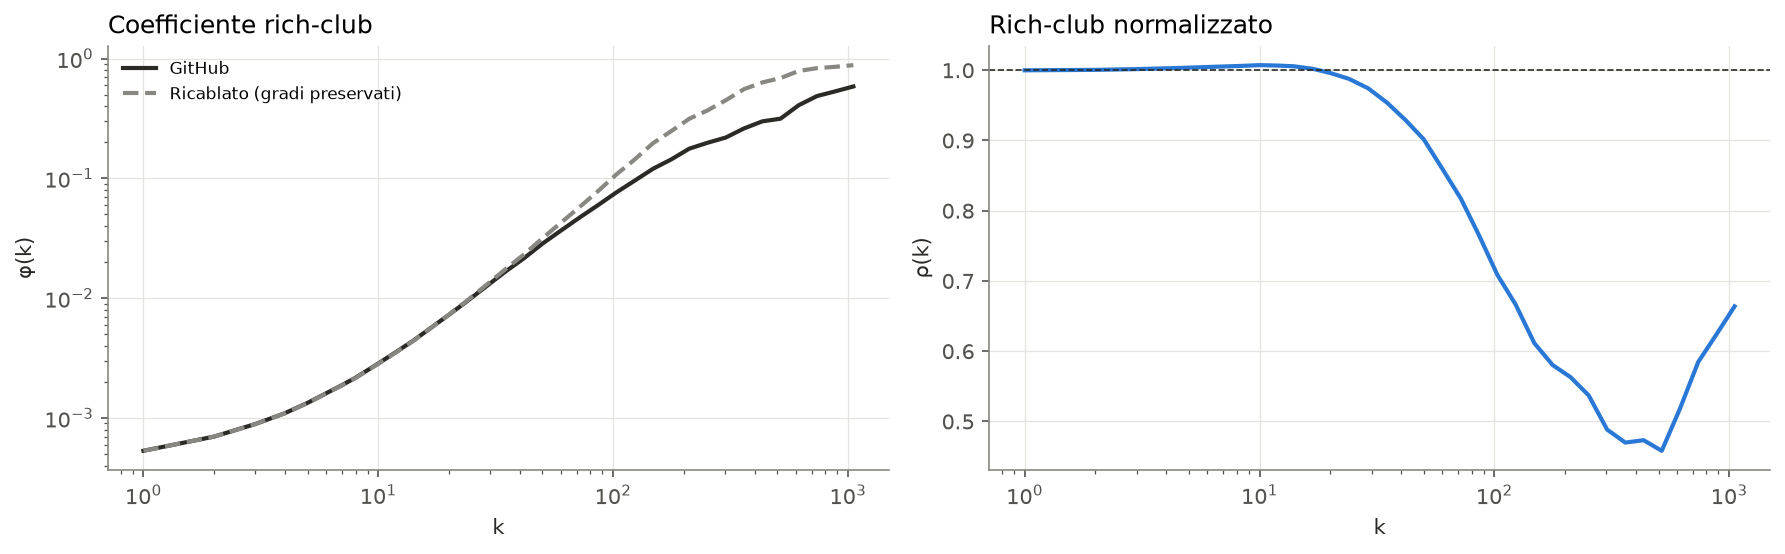
\includegraphics[width=\textwidth]{../3_STRUCTURE_ANALYSIS/figures/04_rich_club.png}
  \caption{A sinistra, coefficiente rich-club della rete reale e dei grafi
  ricablati; a destra, coefficiente normalizzato $\rho(k)$.}
  \label{fig:st_richclub}
\end{figure}

La Figura~\ref{fig:st_richclub} mostra che $\rho(k)\approx 1$ fino a $k\approx 25$
e scende poi sotto 1, fino a un minimo di \num{0.46} per $k=516$: i 70 nodi con più
di 432 vicini sono collegati tra loro con una densità di \num{0.30}, contro
\num{0.63} nei grafi ricablati. La rete quindi \textbf{non ha un rich-club}: gli
hub tendono a evitarsi. È coerente con la disassortatività di grado
(Sezione~\ref{sec:st_smallworld}) e con il fatto che ogni grande hub raccoglie
attorno a sé una propria area della rete, come si vedrà con le community.

% ------------------------------------------------------------
\section{Community detection}
\label{sec:st_community}

Una \textbf{community} è un gruppo di nodi densamente collegati tra loro e
debolmente collegati al resto della rete. La qualità di una suddivisione in
community si misura di solito con la \textbf{modularità}
\[
  Q = \frac{1}{2m}\sum_{i,j}\left[A_{ij} - \gamma\frac{k_i k_j}{2m}\right]\delta(c_i,c_j),
\]
che confronta il numero di archi interni alle community con quello atteso in un
grafo casuale con gli stessi gradi; $c_i$ è la community del nodo $i$ e
$\gamma$ è il parametro di risoluzione (nella modularità standard $\gamma=1$).

\subsection{Algoritmi}
Sono stati confrontati cinque algoritmi:
\begin{itemize}
  \item \textbf{Louvain}: ottimizzazione greedy della modularità in due fasi
        ripetute, spostamento locale dei nodi e aggregazione delle community;
  \item \textbf{Leiden}: miglioramento di Louvain che garantisce community
        connesse internamente, grazie a una fase di raffinamento;
  \item \textbf{Label Propagation}: ogni nodo adotta l'etichetta più frequente tra
        i vicini, fino a convergenza;
  \item \textbf{Infomap}: minimizza la lunghezza della descrizione di una
        passeggiata casuale sulla rete (\emph{map equation});
  \item \textbf{Fast Greedy} (Clauset--Newman--Moore): clustering gerarchico
        agglomerativo che unisce a ogni passo le due community che aumentano di più
        la modularità.
\end{itemize}

\begin{table}[H]
  \centering
  \caption{Confronto tra gli algoritmi di community detection. L'NMI (normalized
  mutual information) misura l'accordo tra la partizione e la classe web/ML.}
  \label{tab:st_algoritmi}
  \small
  \begin{tabular}{@{}lrrrrr@{}}
    \toprule
    \textbf{Algoritmo} & \textbf{Community} & \textbf{Modularità $Q$} & \textbf{Comm.\ max} & \textbf{NMI classe} & \textbf{Tempo (s)} \\
    \midrule
    Louvain           & 30         & \num{0.453} & \SI{22.0}{\percent} & \num{0.115} & \num{0.2} \\
    Leiden            & 30         & \num{0.459} & \SI{19.8}{\percent} & \num{0.112} & \num{2.4} \\
    Label Propagation & 12         & \num{0.000} & \SI{99.9}{\percent} & \num{0.003} & \num{0.1} \\
    Infomap           & \num{1470} & \num{0.394} & \SI{15.2}{\percent} & \num{0.068} & \num{4.8} \\
    Fast Greedy       & 407        & \num{0.393} & \SI{31.0}{\percent} & \num{0.066} & \num{25.6} \\
    \bottomrule
  \end{tabular}
\end{table}

\begin{figure}[H]
  \centering
  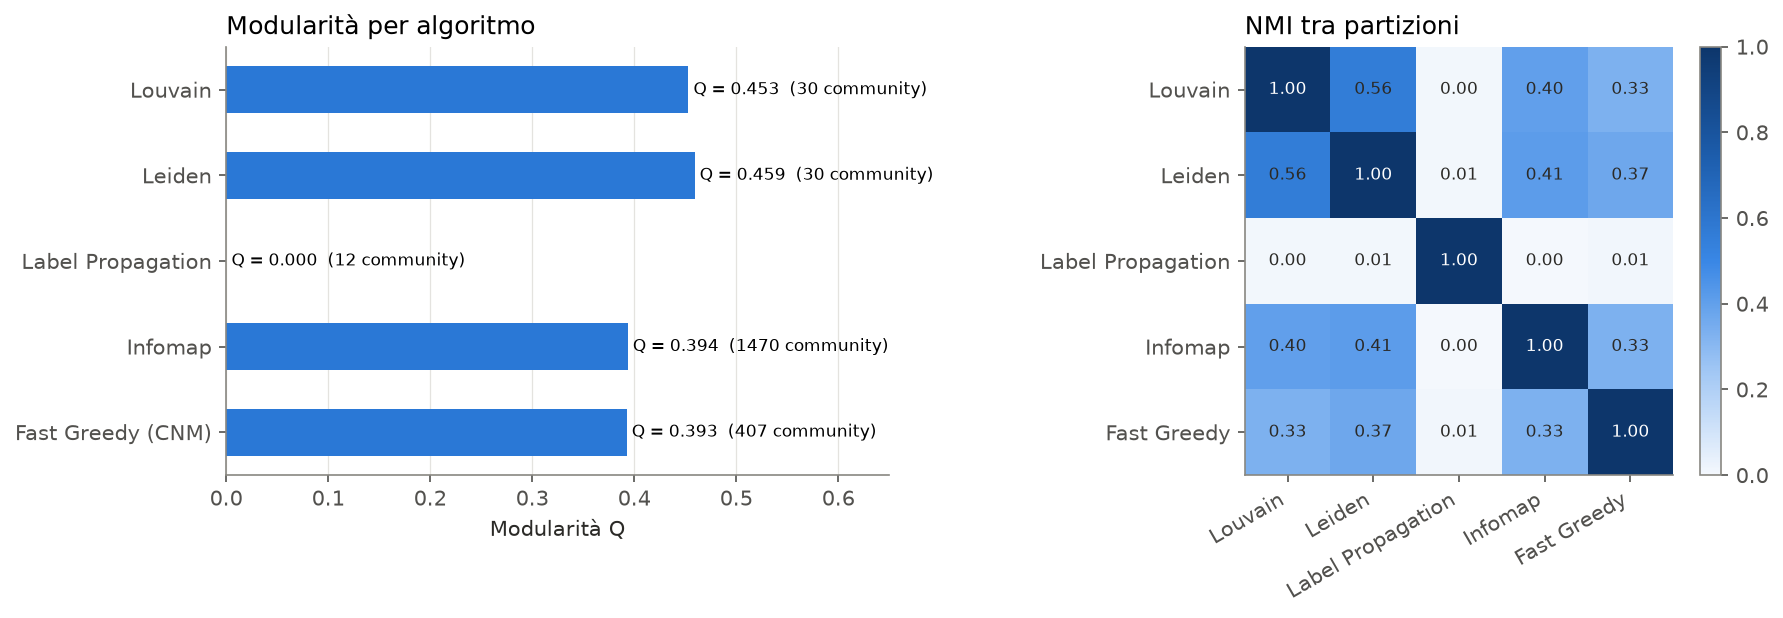
\includegraphics[width=\textwidth]{../3_STRUCTURE_ANALYSIS/figures/05_community_algoritmi.png}
  \caption{A sinistra, modularità ottenuta da ciascun algoritmo; a destra, NMI tra
  le partizioni prodotte dai diversi algoritmi.}
  \label{fig:st_algoritmi}
\end{figure}

Dalla Tabella~\ref{tab:st_algoritmi} e dalla Figura~\ref{fig:st_algoritmi}
emerge quanto segue.
\begin{itemize}
  \item \textbf{Leiden} ottiene la modularità più alta ($Q=\num{0.459}$), seguito
        da Louvain ($Q=\num{0.453}$). Entrambi trovano 30 community, di cui circa
        15 con almeno 10 nodi. Un valore di $Q$ intorno a \num{0.45} indica una
        struttura a community ben definita.
  \item \textbf{Label Propagation fallisce}: mette il \SI{99.9}{\percent} dei nodi
        in un'unica community ($Q\approx 0$). Gli hub, con migliaia di vicini,
        diffondono la propria etichetta a quasi tutta la rete già nelle prime
        iterazioni. È un limite noto dell'algoritmo sulle reti con hub molto
        grandi.
  \item \textbf{Infomap} e \textbf{Fast Greedy} producono partizioni molto più
        frammentate, con centinaia di community piccole, e modularità più bassa.
  \item L'accordo tra gli algoritmi è solo moderato: l'NMI tra Louvain e Leiden è
        \num{0.56}. Con hub che collegano molte aree diverse, l'assegnazione dei
        nodi di confine è ambigua, e algoritmi diversi (o esecuzioni diverse dello
        stesso algoritmo) la risolvono in modo diverso.
\end{itemize}
Nel seguito si utilizza la partizione di Leiden.

\subsection{Effetto della risoluzione}
Il parametro $\gamma$ controlla la scala delle community: valori minori di 1
favoriscono poche community grandi, valori maggiori molte community piccole. La
Tabella~\ref{tab:st_gamma} riporta il risultato di Leiden al variare di $\gamma$.

\begin{table}[H]
  \centering
  \caption{Leiden al variare della risoluzione $\gamma$. La modularità è calcolata
  sempre con $\gamma=1$, per rendere confrontabili i risultati.}
  \label{tab:st_gamma}
  \small
  \begin{tabular}{@{}rrrrr@{}}
    \toprule
    $\gamma$ & \textbf{Community ($\geq 10$ nodi)} & \textbf{Modularità $Q$} & \textbf{Comm.\ max} & \textbf{NMI classe} \\
    \midrule
    \num{0.25} & 1   & \num{0.000} & \SI{99.8}{\percent} & \num{0.004} \\
    \num{0.5}  & 4   & \num{0.379} & \SI{56.5}{\percent} & \num{0.199} \\
    1          & 15  & \num{0.459} & \SI{19.8}{\percent} & \num{0.112} \\
    2          & 42  & \num{0.420} & \SI{8.7}{\percent}  & \num{0.080} \\
    4          & 129 & \num{0.369} & \SI{5.1}{\percent}  & \num{0.062} \\
    8          & 320 & \num{0.296} & \SI{1.9}{\percent}  & \num{0.051} \\
    \bottomrule
  \end{tabular}
\end{table}

La modularità standard è massima per $\gamma=1$. L'accordo con la classe web/ML è
invece massimo per $\gamma=\num{0.5}$ (NMI \num{0.20}): con sole 4 community
grandi, la rete si divide approssimativamente in un'area ML e in aree web. Aumentando
$\gamma$ le community si suddividono in gruppi più piccoli, che non seguono più la
distinzione tra le classi.

\subsection{Le community di Leiden}

\begin{table}[H]
  \centering
  \caption{Le dieci community più grandi trovate da Leiden. La conduttanza è il
  rapporto tra gli archi uscenti e il volume (somma dei gradi) della community: più
  è bassa, più la community è separata dal resto della rete.}
  \label{tab:st_leiden}
  \small
  \begin{tabular}{@{}rlrrrr@{}}
    \toprule
    \textbf{\#} & \textbf{Hub} & \textbf{Nodi} & \textbf{Quota ML} & \textbf{Densità} & \textbf{Conduttanza} \\
    \midrule
    1  & \texttt{nfultz}            & \num{7474} & \SI{74.1}{\percent} & \num{0.0012} & \num{0.30} \\
    2  & \texttt{addyosmani}        & \num{6569} & \SI{5.2}{\percent}  & \num{0.0017} & \num{0.42} \\
    3  & \texttt{gabrielpconceicao} & \num{6246} & \SI{12.1}{\percent} & \num{0.0014} & \num{0.45} \\
    4  & \texttt{ronenhamias}       & \num{5143} & \SI{18.1}{\percent} & \num{0.0027} & \num{0.29} \\
    5  & \texttt{rfthusn}           & \num{2787} & \SI{12.7}{\percent} & \num{0.0035} & \num{0.42} \\
    6  & \texttt{dalinhuang99}      & \num{2650} & \SI{26.7}{\percent} & \num{0.0023} & \num{0.52} \\
    7  & \texttt{philsturgeon}      & \num{2591} & \SI{5.1}{\percent}  & \num{0.0024} & \num{0.45} \\
    8  & \texttt{onevcat}           & \num{1517} & \SI{22.8}{\percent} & \num{0.0059} & \num{0.44} \\
    9  & \texttt{nelsonic}          & 747        & \SI{22.2}{\percent} & \num{0.0030} & \num{0.71} \\
    10 & \texttt{hunkim}            & 567        & \SI{35.3}{\percent} & \num{0.0125} & \num{0.37} \\
    \bottomrule
  \end{tabular}
\end{table}

\begin{figure}[H]
  \centering
  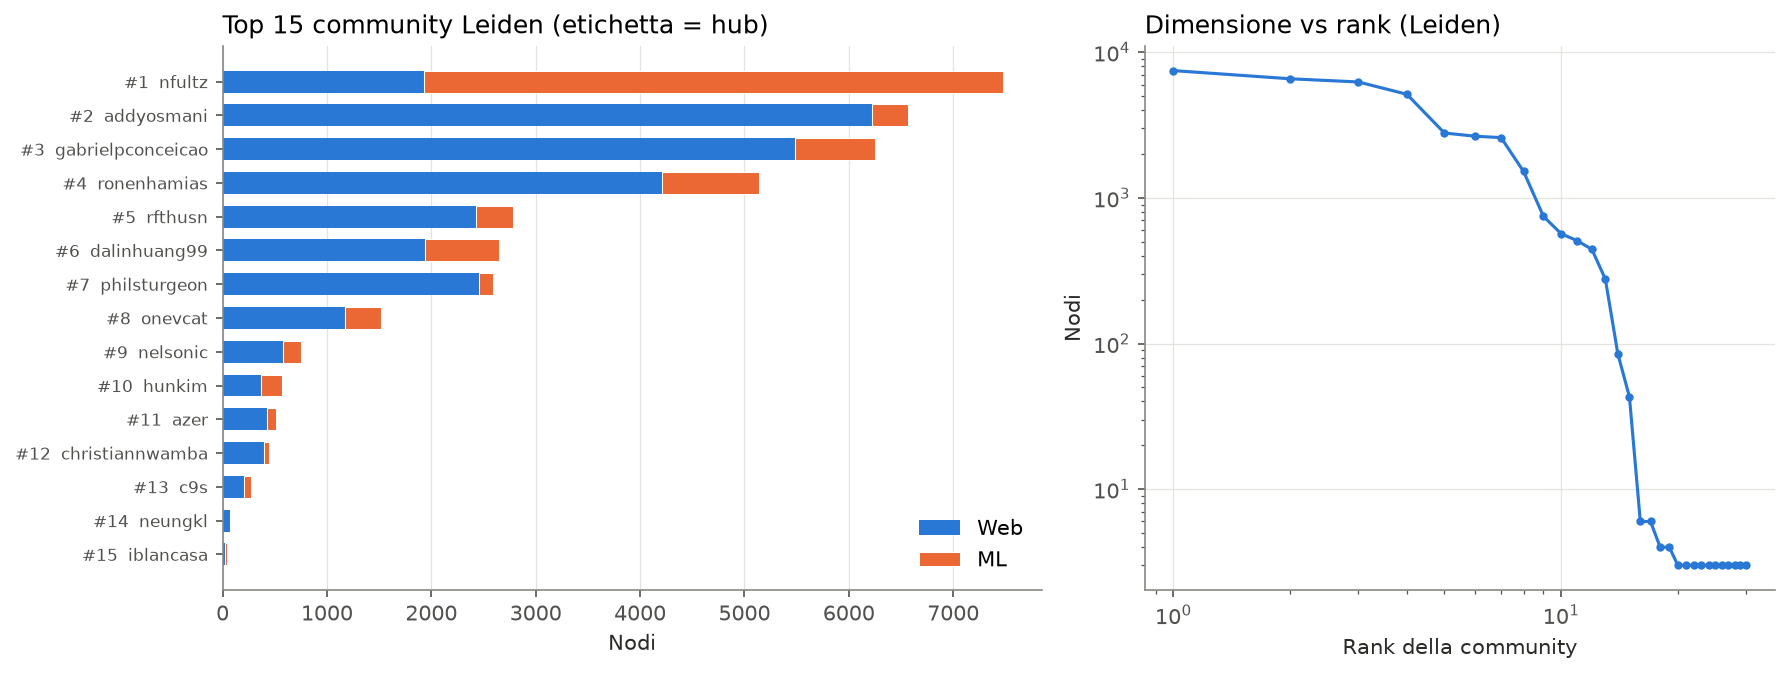
\includegraphics[width=\textwidth]{../3_STRUCTURE_ANALYSIS/figures/06_community_leiden.png}
  \caption{A sinistra, composizione per classe delle 15 community più grandi
  (l'etichetta è l'hub, cioè il nodo di grado massimo, della community); a destra,
  dimensione delle community in funzione del rango.}
  \label{fig:st_leiden}
\end{figure}

\begin{figure}[H]
  \centering
  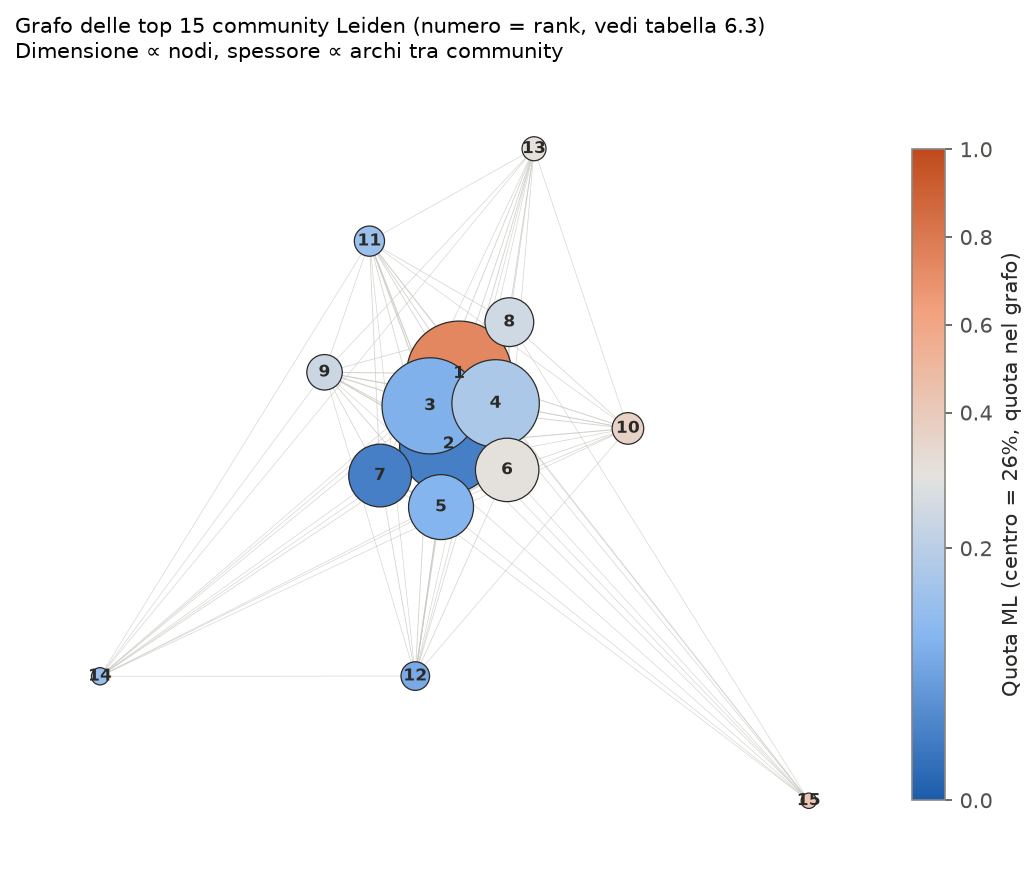
\includegraphics[width=0.8\textwidth]{../3_STRUCTURE_ANALYSIS/figures/07_grafo_community.png}
  \caption{Grafo delle 15 community più grandi: ogni nodo è una community, con
  dimensione proporzionale al numero di sviluppatori; lo spessore degli archi è
  proporzionale al numero di archi tra le community; il colore indica la quota di
  sviluppatori ML (grigio = quota media della rete).}
  \label{fig:st_grafo_community}
\end{figure}

La Tabella~\ref{tab:st_leiden} e le Figure~\ref{fig:st_leiden}
e~\ref{fig:st_grafo_community} mostrano che:
\begin{itemize}
  \item le community sono organizzate \textbf{attorno agli hub}: in cinque delle
        sei community più grandi il nodo di grado massimo è uno dei sei nodi più
        centrali del Capitolo~\ref{cap:centralita}. Le prime 15 community coprono il
        \SI{99.9}{\percent} dei nodi, e le loro dimensioni decrescono rapidamente
        con il rango;
  \item esiste una \textbf{community ML}: la community 1 (\num{7474} nodi) è
        composta per il \SI{74}{\percent} da sviluppatori ML e contiene il
        \SI{57}{\percent} di tutti gli sviluppatori ML della rete. Il suo hub,
        \texttt{nfultz}, il secondo nodo più centrale della rete, è invece
        classificato come sviluppatore web. È anche una delle community più
        separate dal resto (conduttanza \num{0.30});
  \item le altre nove community più grandi sono prevalentemente web, con quote ML
        tra il \SI{5}{\percent} e il \SI{35}{\percent};
  \item la community di \texttt{dalinhuang99}, l'hub più grande della rete, ha la
        conduttanza più alta tra le prime otto (\num{0.52}): circa metà dei suoi archi
        esce dalla community, coerentemente con il ruolo di ponte tra aree diverse
        emerso dalla betweenness.
\end{itemize}

Per quantificare il legame tra community e classe si può usare l'entropia. Senza
informazioni, l'incertezza sulla classe di uno sviluppatore è $H=\num{0.824}$ bit;
conoscendo la sua community scende in media a \num{0.600} bit. La community spiega
quindi il \SI{27}{\percent} dell'incertezza sulla classe. È un legame chiaro ma
parziale: la rete separa bene l'area ML, ma una parte degli sviluppatori ML (circa
il \SI{43}{\percent}) è distribuita nelle community web.

% ------------------------------------------------------------
\section{Visualizzazione della rete}
\label{sec:st_visualizzazione}

Per visualizzare l'intera rete si è utilizzato l'algoritmo di layout
\textbf{DrL} (Distributed Recursive Layout), un algoritmo \emph{force-directed}
progettato per grafi di grandi dimensioni: nodi collegati si attraggono, nodi non
collegati si respingono, e i gruppi densi risultano quindi vicini nel disegno. Il
calcolo del layout richiede circa due minuti. Per leggibilità sono disegnati tutti i
nodi, con dimensione proporzionale alla radice del grado, ma solo un campione
casuale di \num{60000} archi.

\begin{figure}[H]
  \centering
  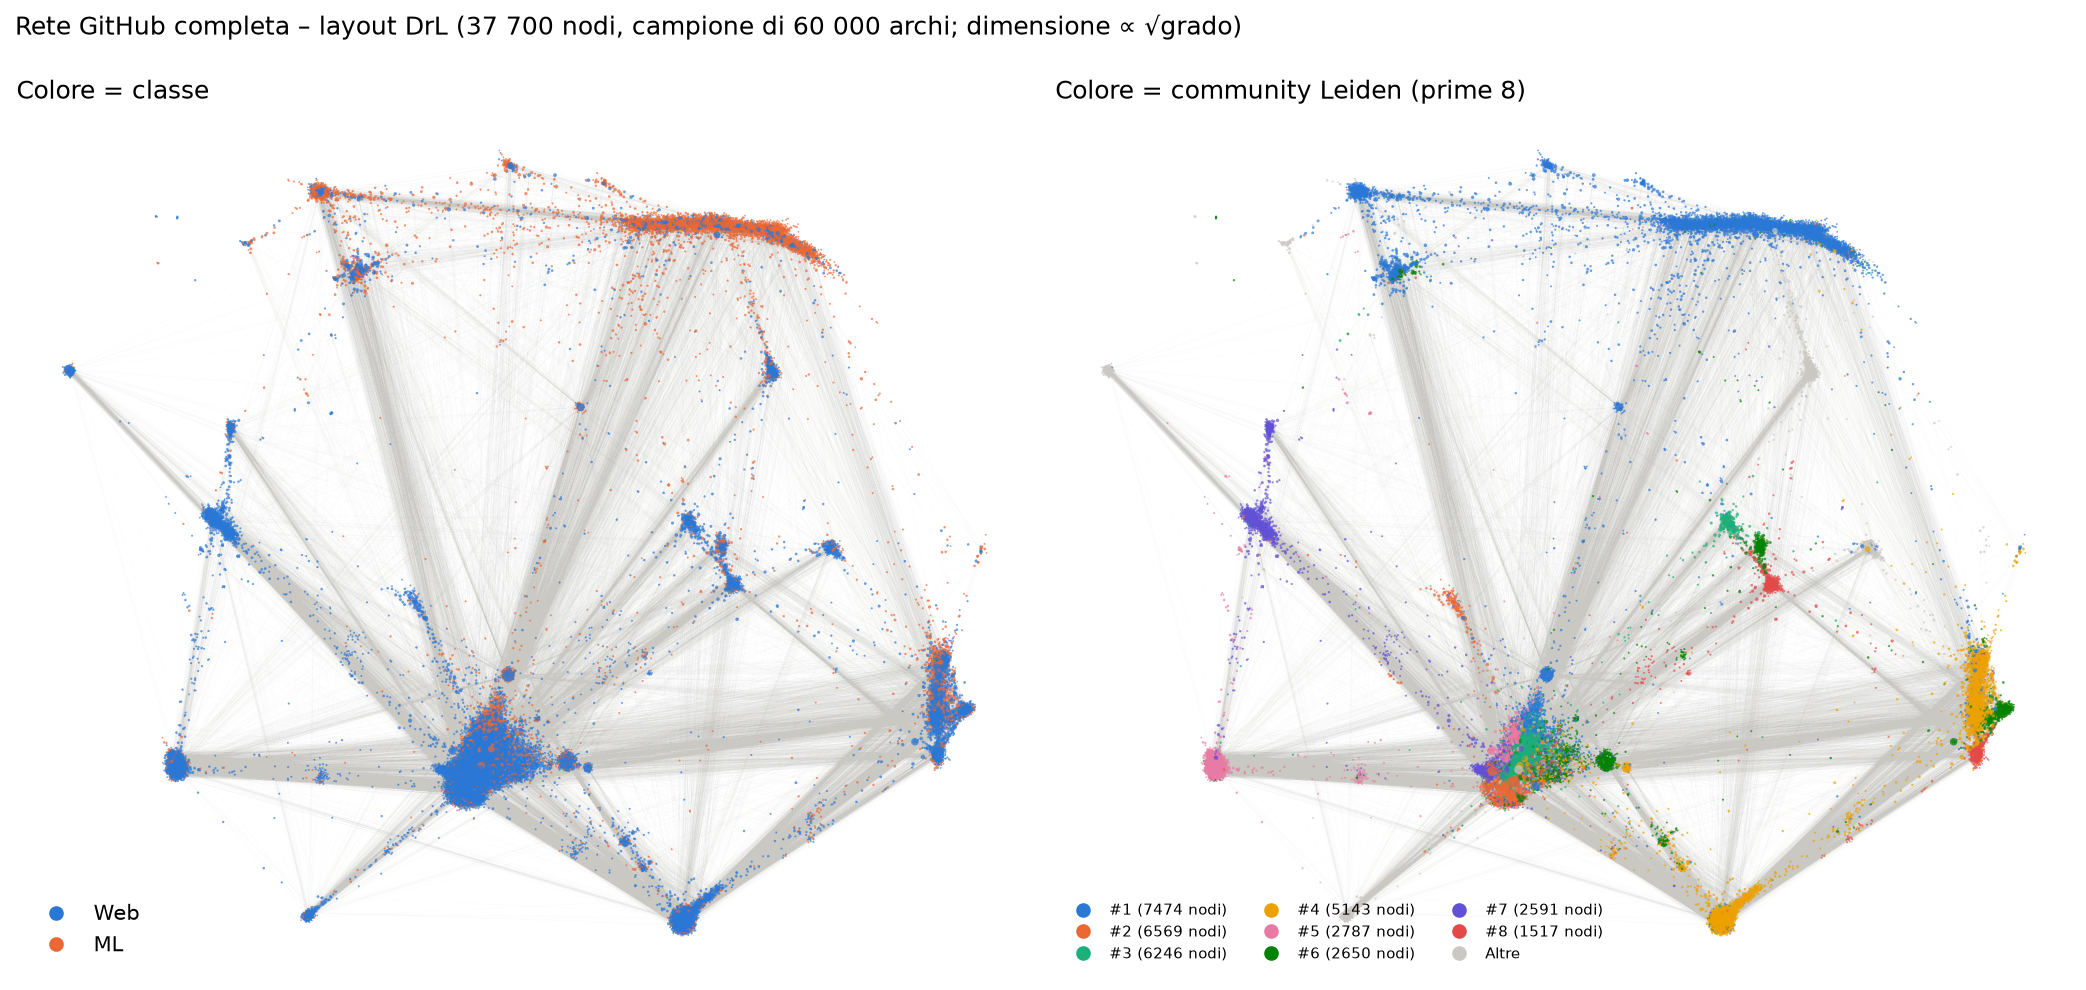
\includegraphics[width=\textwidth]{../3_STRUCTURE_ANALYSIS/figures/08_rete_completa.png}
  \caption{La rete completa con layout DrL. A sinistra i nodi sono colorati per
  classe, a destra per community di Leiden (le otto più grandi; in grigio le
  altre).}
  \label{fig:st_rete}
\end{figure}

La Figura~\ref{fig:st_rete} riassume visivamente i risultati del capitolo:
\begin{itemize}
  \item la rete è formata da diversi \textbf{gruppi densi}, ciascuno raccolto
        attorno a uno o più hub e collegato agli altri da fasci di archi;
  \item gli \textbf{sviluppatori ML} (in arancione a sinistra) sono concentrati in
        un'area ben distinta nella parte alta del disegno, che corrisponde alla
        community 1 di Leiden; altri sviluppatori ML sono sparsi nelle aree web;
  \item le community di Leiden (a destra) corrispondono in larga parte ai gruppi
        visibili nel layout, che è calcolato in modo indipendente: è una conferma
        qualitativa della partizione trovata.
\end{itemize}

% ------------------------------------------------------------
\section{Conclusioni}
\label{sec:st_conclusioni}

\begin{itemize}
  \item La rete ha una struttura \textbf{nucleo--periferia}: un nucleo biconnesso
        con l'\SI{86}{\percent} dei nodi, un nucleo interno di 360 nodi
        (34-core) e una periferia di nodi collegati alla rete da un solo arco.
  \item È una rete \textbf{small-world} con \textbf{struttura gerarchica}: distanze
        brevi, clustering molto superiore a quello di un grafo casuale e decrescente
        con il grado. Distanze e disassortatività sono spiegate dalla distribuzione
        dei gradi; il clustering no.
  \item \textbf{Non c'è un rich-club}: gli hub non si collegano tra loro più del
        caso, ma ciascuno organizza attorno a sé una propria area della rete.
  \item La rete ha una chiara \textbf{struttura a community}
        ($Q=\num{0.459}$ con Leiden), con community organizzate attorno agli hub.
        Label Propagation fallisce su questa rete a causa degli hub molto grandi.
  \item La struttura riflette in parte la \textbf{classe degli sviluppatori}: esiste
        una community ML che raccoglie il \SI{57}{\percent} degli sviluppatori ML,
        mentre il nucleo della rete è quasi esclusivamente web
        (\SI{1.4}{\percent} ML nel 34-core).
\end{itemize}

% ==================== CAPITOLO 5 - Link Prediction nei Grafi ====================
\chapter{Link Prediction nei Grafi}
\label{cap:link_prediction}


\chapter{CONCLUSIONI}

% -------------------- Bibliografia --------------------
\bibliographystyle{ieeetr}
\bibliography{bibl}

\end{document}
